%%%%%%%%%%%%%%%%%%%%%%%%%%%%%%%%%%%%%%
%%    UNIVERSIDADE DE ITAUNA        %%
%%  Autor: Zilton Cordeiro Junior   %%
%%  Vers�o: 1.1                     %%
%%  Data: Fevereiro/2014            %%
%%%%%%%%%%%%%%%%%%%%%%%%%%%%%%%%%%%%%%
% --- -----------------------------------------------------------------
% --- Arquivo principal. Os demais serao os dos capitulos.
% --- -----------------------------------------------------------------

\documentclass[ruledheader, a4paper]{abnt_UFF}

%---pacotes para hipheniza��o e acentua��o em portugues
\usepackage[brazil]{babel}
\usepackage[T1]{fontenc}
\usepackage{hyperref}
\usepackage{url}
%--- pacote para figuras
\usepackage{epsf}
%--- pacote para incluir figuras
\usepackage[]{graphicx}
\usepackage[normalem]{ulem} 
%--- pacote de simbolos
\usepackage{latexsym}
%--- simbolos matematicos
\usepackage{amsmath}
\usepackage{amssymb}
%--- pacote para algoritmos
\usepackage{algorithmic}
%--- pacote para tabelas landscape
\usepackage{rotating}
\usepackage{multirow}
\usepackage[nottoc,notlof,notlot]{tocbibind}
\usepackage{listings}
\usepackage[final]{pdfpages}
\hyphenation{pes-qui-sa-do-res}
% Tabelas com qualidade de publicacao
\usepackage{booktabs}
%\usepackage{lscape}
\usepackage{pdflscape}
\usepackage{graphicx}
\usepackage{caption}
\usepackage{subcaption}
\usepackage[boxed,portugues,linesnumbered]{algorithm2e}
%--- pacote para exibi��o de trecho de c�digo fonte
\usepackage{listings}
\definecolor{mygreen}{rgb}{0,0.6,0}
\definecolor{mygray}{rgb}{0.5,0.5,0.5}
\definecolor{mymauve}{rgb}{0.58,0,0.82}

\lstset{ %
   backgroundcolor=\color{white},   % choose the background color; you must add \usepackage{color} or \usepackage{xcolor}
   basicstyle=\footnotesize,        % the size of the fonts that are used for the code
   breakatwhitespace=false,         % sets if automatic breaks should only happen at whitespace
   breaklines=true,                 % sets automatic line breaking
   captionpos=b,                    % sets the caption-position to bottom
   commentstyle=\color{mygreen},    % comment style
   deletekeywords={...},            % if you want to delete keywords from the given language
   escapeinside={\%*}{*)},          % if you want to add LaTeX within your code
   extendedchars=true,              % lets you use non-ASCII characters; for 8-bits encodings only, does not work with UTF-8
   %frame=single,                    % adds a frame around the code
   keepspaces=true,                 % keeps spaces in text, useful for keeping indentation of code (possibly needs columns=flexible)
   keywordstyle=\color{blue},       % keyword style
   language=C++,                 % the language of the code
   morekeywords={*,...},            % if you want to add more keywords to the set
   numbers=left,                    % where to put the line-numbers; possible values are (none, left, right)
   numbersep=5pt,                   % how far the line-numbers are from the code
   numberstyle=\tiny\color{mygray}, % the style that is used for the line-numbers
   rulecolor=\color{black},         % if not set, the frame-color may be changed on line-breaks within not-black text (e.g. comments (green here))
   showspaces=false,                % show spaces everywhere adding particular underscores; it overrides 'showstringspaces'
   showstringspaces=false,          % underline spaces within strings only
   showtabs=false,                  % show tabs within strings adding particular underscores
   stepnumber=1,                    % the step between two line-numbers. If it's 1, each line will be numbered
   stringstyle=\color{mymauve},     % string literal style
   tabsize=2,                       % sets default tabsize to 2 spaces
   %title=\lstname                   % show the filename of files included with \lstinputlisting; also try caption instead of title
}

%---------usando tipo de fonte padrao
\renewcommand{\ABNTchapterfont}{\bfseries\fontfamily{cmr}\fontseries{b}\selectfont}
\renewcommand{\ABNTsectionfont}{\bfseries\fontfamily{cmr}}

% --- -----------------------------------------------------------------
% --- Documento Principal.
% --- -----------------------------------------------------------------
\begin{document}

% --- -----------------------------------------------------------------
% --- Titulo, abstract, dedicatorias e agradecimentos.
% --- Indice geral, lista de figuras e tabelas.
% --- -----------------------------------------------------------------

% --- -----------------------------------------------------------------
% --- Elementos usados na Capa e na Folha de Rosto.
% --- -----------------------------------------------------------------

% >>>>>>>>>>>>>>>>>>>>>>>>>>>>>>>>> BLOCO A SER ALTERADO >>>>>>>>>>>>>>>>>>>>>>>>>>>>>>>>>>>>>>>>>>>>>>
\autor{MICHAEL DOUGRAS DA SILVA } % deve ser escrito em mai�sculo

\titulo{ORM4Qt: Biblioteca de Mapeamento Objeto Relacional em C++ para o Framework Qt}

\instituicao{UNIVERSIDADE DE ITA�NA \par FACULDADE DE ENGENHARIA \par CI�NCIA DA COMPUTA��O}

\orientador{Ang�lica Aparecida Moreira}

%\coorientador{Sicrano de Tal} % se n�o existir co-orientador comente essa linha

\local{Ita�na}

\data{2014} % ano da defesa

% >>>>>>>>>>>>>>>>>>>>>>>>>>>>>>>>> FIM DO BLOCO A SER ALTERADO >>>>>>>>>>>>>>>>>>>>>>>>>>>>>>>>>>>>>>>


\comentario{Trabalho de Conclus�o de Curso apresentado
como requisito parcial para obten��o do t�tulo
de Bacharel em Ci�ncia da Computa��o da Faculdade
de Engenharia da Universidade de Ita�na.}

% --- -----------------------------------------------------------------
% --- Capa externa
% --- ----------------------------------------------------------------
\capa

% --- -----------------------------------------------------------------
% --- Folha de rosto. (Obrigatorio)
% --- ----------------------------------------------------------------
\folhaderosto
\pagestyle{ruledheader}
\setcounter{page}{1}
\pagenumbering{roman}

% --- -----------------------------------------------------------------
% --- Termo de aprovacao. (Obrigatorio)
% --- ----------------------------------------------------------------
  \cleardoublepage
  \thispagestyle{empty}
  \vspace{-60mm}

  %T�tulo do TCC
  \begin{center} {\large ORM4Qt: Biblioteca de Mapeamento Objeto Relacional em C++ para o Framework Qt}\\
      \vspace{7mm}
      Michael Dougras da Silva\\ % Nome do Aluno
      \vspace{10mm}
  \end{center}
  \noindent

  \begin{flushright}
  \begin{minipage}[t]{8cm}
      Este trabalho foi julgado adequado para obten��o da aprova��o na disciplina Trabalho de Conclus�o do Curso de Ci�ncia da Computa��o
da Faculdade de Engenharia da Universidade de Ita�na.
  \end{minipage}
  \end{flushright}
  \vspace{1cm}
  \noindent  
  Aprovado por:\\

  \begin{flushright}
    \parbox{13cm}{
	\begin{center}
	    %Altere o nome dos membros da banca, orientador e co-orientador, quando necess�rio.
	    %Caso seja necess�rio adicionar mais membros ou remover, manipule o bloco de tr�s linhas,
	    %conforme os tr�s blocos abaixo.
	    \rule{13cm}{.1mm} \\
	    Ang�lica Aparecida Moreira
	    \vspace{6mm}

	    %Caso voc� n�o tenha co-orientador, favor remover.
	    %\rule{13cm}{.1mm} \\
	    %Sicrano de Tal, Titula��o/Institui��o\\ (Co-orientador)\\
	    %\vspace{6mm}

	    \rule{13cm}{.1mm} \\
	    Paulo de Tarso Gomide Castro Silva
	    \vspace{6mm}
	\end{center}
    }
  \end{flushright}

  %Altere a data abaixo, que � referente ao dia da sua defesa.
  \begin{center}
    \vspace{6mm}
    Ita�na, 05 de Junho de 2014.
  \end{center}



% --- -----------------------------------------------------------------
% --- Dedicatoria. (Opcional)
% --- -----------------------------------------------------------------
%\cleardoublepage
%\thispagestyle{empty}
%\vspace*{170mm}
%\begin{flushright}\small{
  {
    \em Dedico este trabalho...
  }
}\end{flushright}

% --- -----------------------------------------------------------------
% --- Agradecimentos. (Opcional)
% --- -----------------------------------------------------------------
%\newpage
%\pretextualchapter{Agradecimentos}
%\hspace{5mm}
%Agrade\c{c}o primeiramente a...


% --- -----------------------------------------------------------------
% --- Resumo em portugues.(Obrigatorio)
% --- -----------------------------------------------------------------
\begin{resumo}
As Linguagens Orientadas a Objetos em conjunto com os Sistemas Gerenciadores de Bancos de Dados Relacionais (SGBDs) s�o considerados padr�es no desenvolvimento de Sistemas de Informa��o Empresarial. Embora o uso destas duas tecnologias em conjunto mostre resultados satisfat�rios, encontra-se dificuldade em efetuar a transi��o de informa��es entre os seus contextos de representa��o de dados.

Para efetuar a transi��o de informa��es � necess�rio desenvolver componentes de \textit{software} espec�ficos para cada classe que represente dados que necessitam ser persistidos no banco de dados, o que se mostra uma tarefa repetitiva e propensa a erros.
Com o objetivo de amenizar este problema, foram criadas as Bibliotecas de Mapeamento Objeto Relacional (ORMs), que s�o componentes de \textit{software} capazes de automatizar o processo de transi��o de dados entre os dois contextos.

Devido a limita��es nos recursos de reflex�o e inser��o de metadados oferecidos pela linguagem C++, o desenvolvimento de solu��es ORM para esta linguagem se mostra uma tarefa bastante complexa. A maioria das solu��es implementadas apresenta interfaces de configura��o complexas, al�m de utilizar recursos da linguagem que promovem o aumento do n�vel de acoplamento do c�digo.

Este trabalho prop�e o desenvolvimento de uma biblioteca ORM para a linguagem C++, onde s�o implementados mecanismos pr�prios de reflex�o e inser��o de metadados a partir da utiliza��o dos novos recursos propostos pela especifica��o \textit{C++11}. A biblioteca utiliza v�rios componentes oferecidos pelo \textit{framework} Qt para auxiliar em tarefas como comunica��o com banco de dados e extens�o de tipos nativos. 


{\bf{Palavras-chave}}: Orienta��o a Objetos, SGBD, C++, ORM


\end{resumo}

% --- -----------------------------------------------------------------
% --- Resumo em lingua estrangeira.(Opcional)
% --- -----------------------------------------------------------------
\begin{abstract}
LaTeX is a document preparation system and document markup language. LaTeX uses the TeX typesetting program for formatting its output, and
is itself written in the TeX macro language. LaTeX is not the name of a particular editing program, but refers to the encoding or tagging
conventions that are used in LaTeX documents. Almost any editing program or word-processor may be used to write LaTeX documents, although
there are many editing programs written specially to make using LaTeX easy. Interactive websites and smartphone apps are increasingly (2013)
generalizing and simplifying the tasks of writing documents with LaTeX.

LaTeX is widely used in academia. It is also used as the primary method of displaying formulas on Wikipedia. LaTex can be used as a
primary or intermediate format, e.g., translating DocBook and other XML-based formats to PDF. The typesetting system offers programmable
desktop publishing features and extensive facilities for automating most aspects of typesetting and desktop publishing, including numbering
and cross-referencing, tables and figures, page layout and bibliographies.

Like TeX, LaTeX started as a writing tool for mathematicians and computer scientists. But from early in its development it was also taken up
by scholars who needed to write documents that included complex non-Latin scripts, such as Arabic, Sanskrit and Chinese.

LaTeX is intended to provide a high-level language that accesses the power of TeX. LaTeX essentially comprises a collection of TeX macros
and a program to process LaTeX documents. Because the TeX formatting commands are very elementary, it offers authors ready-made commands for
common requirements such as chapter headings, footnotes, cross-references and bibliographies.

LaTeX was originally written in the early 1980s by Leslie Lamport at SRI International. The current version is LaTeX2e (styled as
LATEX2ε). LaTeX is free software and is distributed under the LaTeX Project Public License (LPPL).

{\bf{Keywords}}: UIT, LATEX, Computer Science
\end{abstract}

% --- -----------------------------------------------------------------
% --- Gloss�rio com uma lista de abreviacoes.(Opcional)
% --- ----------------------------------------------------------------
\cleardoublepage
\pretextualchapter{Gloss\'ario}
\begin{tabular}{lcl}

API & : & \textit{Application Programming Interface};\\
ORM & : & \textit{Object Relational Mapping};\\
SGBD & : & Sistema Gerenciador de Banco de Dados;\\
SQL & : & \textit{Structured Query Language};\\
\end{tabular}


% --- -----------------------------------------------------------------
% --- Sumario.(Obrigatorio)
% --- -----------------------------------------------------------------
\pagestyle{ruledheader}
\tableofcontents

% --- -----------------------------------------------------------------
% --- Lista de figuras.(Opcional)
% --- -----------------------------------------------------------------
\listoffigures


% --- -----------------------------------------------------------------
% --- Lista de tabelas.(Opcional)
% --- -----------------------------------------------------------------
%\listoftables
\listofalgorithms
\cleardoublepage


% --- -----------------------------------------------------------------
% --- Insercao dos capitulos.
% --- Aqui voce deve alterar:
% --- --- os nomes dos capitulos (\chapter{})
% --- --- o marcador para referencia (\label{})
% --- --- o nome do arquivo de entrada, mantendo a extensao .tex (\input{})
% --- -----------------------------------------------------------------
\pagestyle{ruledheader}
\setcounter{page}{1}
\pagenumbering{arabic}

%-------------------------------------------------------------
\chapter{Introdu��o}
\label{chap:cap1}
% Contexto %

Vivemos em uma era onde os sistemas informatizados deixaram de ser vistos como meras ferramentas de automatiza��o de tarefas. Onde o \textit{software} desempenha papel fundamental no planejamento estrat�gico e desempenho de atividades nas grandes empresas. A prolifera��o de \textbf{Sistemas de Informa��o Empresarial} (\textit{Enterprise Information Systems} - EIS) se mostra cada vez mais not�ria. Estes sistemas s�o caracterizados por sua alta complexidade e por trabalharem com gerenciamento constante de dados \cite{expertCSharpObjects}. 

As \textbf{Linguagens Orientadas a Objetos} se tornaram um padr�o consolidado no desenvolvimento destes sistemas. Devido � sua capacidade de abstrair representa��es de entidades do mundo real como componentes de software, estas linguagens permitem aos arquitetos e engenheiros de \textit{software} terem uma vis�o de alto n�vel durante o planejamento e especifica��o do sistema \cite{oopSurvey}.

Os \textbf{Sistemas Gerenciadores de Bancos de Dados Relacionais}  (\textbf{SGBDs}) s�o o meio consolidado para armazenamento de dados estruturados. Eles permitem o armazenamento de informa��es de tal forma que estas podem ser manipuladas atrav�s de comandos em linguagem \textbf{SQL} ou \textbf{\textit{Structured Query Language}}. Esta linguagem permite executar opera��es de inser��o, remo��o, edi��o e gera��o de consultas de alta complexidade nos dados armazenados \cite{ormPaper}.

Apesar de as linguagens orientadas a objetos serem utilizadas em conjunto com os SGBDs no desenvolvimento de sistemas, a forma de representa��o dos dados nos dois contextos � diferente. No contexto orientado a objetos, as informa��es s�o vistas sobre uma perspectiva comportamental, onde os componentes do \textit{software} s�o importantes n�o somente pelos dados que eles cont�m, mas pela habilidade de se comunicar com outros componentes para compartilhar estas informa��es e executar a��es sobre elas. J� no contexto dos SGBDs, as informa��es s�o vistas sobre uma perspectiva estrutural, onde o objetivo principal das entidades � armazenar os dados e representar suas rela��es da forma mais otimizada poss�vel. N�o existe a preocupa��o em se definir o comportamento das informa��es. Devido a essa diferen�a de representa��o de dados entre os dois contextos, existe a necessidade de convers�o ou mapeamento durante a transi��o entre eles. A gera��o de c�digo para mapeamento se mostra uma tarefa repetitiva e propensa a erros.

Com o objetivo de otimizar a utiliza��o das linguagens orientadas a objetos em conjunto com os SGBDs surgiu o conceito de \textbf{Biblioteca de Mapeamento Objeto Relacional} ou \textbf{ORM} (\textit{Object Relational Mapping}). Este tipo de biblioteca tem como objetivo automatizar as tarefas de mapeamento dos dados entre os dois contextos. Sua utiliza��o promove maior produtividade e redu��o da complexidade envolvida em tarefas de manuten��o e modifica��o do c�digo \cite{ormPaper}. Neste trabalho � proposto o desenvolvimento de uma biblioteca ORM para a linguagem C++. O \textbf{\textit{framework} Qt} � utilizado como aux�lio para comunica��o com os SGBDs, e extens�o dos tipos nativos da linguagem C++. 


%-------------------------------------------------------------
% \chapter{Conceitos b�sicos}
 \chapter{Fundamenta��o Te�rica}
 \label{chap:cap2}
 Neste cap�tulo s�o apresentados os conceitos b�sicos utilizados ao longo do trabalho, situando-os dentro do problema a ser resolvido.

%--- Inserir os conceitos de orienta��o a objetos
\section{Orienta��o a Objetos}
\label{sec:oop}
Um conceito bastante difundido tanto no meio acad�mico quanto no mercado s�o as \textbf{Linguagens Orientadas a Objetos}, que s�o linguagens de programa��o que utilizam um paradigma ou padr�o de estrutura��o de c�digo que permite que o desenvolvedor crie abstra��es no contexto do software para modelar objetos ou entidades do mundo real \cite{oopSurvey}.

N�o existe uma defini��o universal que diga quais s�o as caracter�sticas ou funcionalidades que uma linguagem de programa��o deve apresentar para ser considerada orientada a objetos \cite{oopSurvey}. Por�m, de maneira geral, elas possuem mecanismos que permitem agrupar dentro de uma unidade de \textit{software}, estruturas para prover informa��es de \textbf{estado}, \textbf{comportamento} e \textbf{identidade} \cite{ormPaper}. Este agrupamento de estruturas dentro de uma unidade � conhecido como \textbf{encapsulamento}.

Esta unidade de \textit{software} que representa o estado, comportamento e identidade de uma entidade � conhecida como \textbf{objeto}. Um objeto � criado a partir de um modelo preestabelecido que define todas as estruturas internas que o comp�e. Este modelo � conhecido como \textbf{classe} \cite{oopSurvey}. Algumas linguagens n�o oferecem mecanismos expl�citos para cria��o de classes, por�m oferecem suporte � instancia��o de objetos. Um exemplo de linguagem que apresenta esta caracter�stica � a linguagem \textbf{\textit{Javascript}}\footnote{Linguagem interpretada com tipagem din�mica baseada em \textit{scripts} muito utilizada em programa��o para a WEB e como complemento para interfaces com linguagens e/ou programas complexos.}. 

O estado de um objeto � definido a partir da adi��o de vari�veis em sua estrutura interna para armazenamento de valores. Estes valores podem ser unit�rios (onde s�o armazenados dados do tipo texto ou num�rico, por exemplo), ou podem ser compostos (onde s�o utilizados outros objetos para compor a estrutura interna). As vari�veis internas de um objeto s�o conhecidas como \textbf{atributos} ou \textbf{propriedades} e a utiliza��o de valores compostos na defini��o da estrutura de uma classe � um mecanismo conhecido como \textbf{composi��o} \cite{oopSurvey}. 

O comportamento de um objeto � definido a partir da adi��o de fun��es em sua estrutura interna. Elas s�o utilizadas para efetuar opera��es sobre os atributos que o objeto cont�m, ou para efetuar processamento de dados baseados no estado ou objetivo do objeto ao qual ela pertence. Estas fun��es s�o conhecidas como \textbf{m�todos} \cite{oopSurvey}.

O conjunto de atributos e m�todos de uma classe define o que chamamos de \textbf{interface}. Algumas linguagens permitem reduzir a interface de um objeto de forma que nem todas as estruturas internas sejam acess�veis externamente. Um exemplo � a linguagem C++, que nos permite utilizar os modificadores \textit{\textbf{"private"}} (estruturas n�o acess�veis externamente) e \textit{\textbf{"public"}} (estruturas acess�veis externamente). 

A identidade de um objeto se refere � capacidade de se referenciar inst�ncias de objetos de maneira un�voca, ou seja, se refere � capacidade de se distinguir diversas inst�ncias de objetos entre si atrav�s de algum mecanismo de compara��o \cite{oopSurvey}. Em algumas linguagens este mecanismo se baseia no endere�amento de mem�ria ocupado pela inst�ncia do objeto, como � o caso da linguagem C++. J� em outras linguagens existem mecanismos que permitem a cria��o de fun��es de compara��o, como acontece por exemplo na linguagem \textbf{\textit{JAVA}} onde podemos definir o m�todo \textbf{\textit{"equals"}} das classes criadas. 

Um exemplo de defini��o de uma classe utilizando a linguagem C++ � apresentado no trecho de c�digo  \ref{lst:simpleclass}, para demonstrar os conceitos explicados anteriormente. No c�digo � definida a estrutura de uma classe que representa uma pessoa. A classe foi definida com o identificador Pessoa (linha 1), possui dois atributos internos para armazenar o nome e sobrenome (linhas 3 e 4) e um m�todo que retorna o nome completo de uma pessoa atrav�s da combina��o do seu nome e sobrenome (linha 6). Os atributos n�o s�o acess�veis externamente devido ao modificador de acesso \textit{"private"} utilizado na linha 2. J� o m�todo � acess�vel devido ao modificador de acesso \textit{"public"} utilizado na linha 5.

\begin {algorithm}
\caption{Defini��o de uma classe simples em C++}
\label{lst:simpleclass}
\begin{lstlisting}[]
class Pessoa {
	private:
		string m_nome;
		string m_sobrenome;
	public:
		string nomeCompleto() { return m_nome + m_sobrenome; }
}
\end{lstlisting}
\end{algorithm}

Mecanismos de encapsulamento (m�todos, atributos e restri��o de interface), defini��o de classes e instancia��o de objetos s�o as caracter�sticas mais comumente encontradas nas linguagens consideradas como orientadas a objetos. Por�m, existem mecanismos mais avan�ados que permitem uma melhoria na defini��o do comportamento das classes e promovem reaproveitamento de c�digo. Entre os principais est�o a \textbf{heran�a} e o \textbf{polimorfismo} \cite{oopSurvey}. 

A heran�a consiste na capacidade de uma classe estender a estrutura de uma classe j� definida. Isso significa que a nova classe mant�m a interface da  anterior e tem a capacidade de adicionar novos atributos e m�todos a ela \cite{oopSurvey}. Algumas linguagens oferecem somente suporte para heran�a simples, onde uma classe pode herdar de somente uma outra classe, por�m geralmente definem mecanismos alternativos de extens�o. Um exemplo � a linguagem JAVA. Outras linguagens oferecem suporte para heran�a m�ltipla, onde uma classe pode estender as funcionalidades de uma ou mais classes j� definidas. Um exemplo de linguagem com esta caracter�stica � a linguagem C++.

Algumas nota��es s�o utilizadas para demonstrar a utiliza��o do mecanismo de heran�a. Por exemplo, quando criamos uma classe ``B'' que herda de uma classe ``A'', dizemos que ``A'' � a classe \textbf{base} ou \textbf{pai}, enquanto a ``B'' � uma classe \textbf{especializada} ou \textbf{filha}. Uma caracter�stica importante a observar � que ao declararmos um objeto da classe ``B'', este objeto poder� ser utilizado em contextos onde � esperado um objeto da classe ``A'' \cite{oopSurvey}.

Ao utilizar o mecanismo de heran�a, algumas linguagens permitem a modifica��o de um m�todo existente na classe base. Este mecanismo � utilizado para especializar o comportamento herdado na nova classe, mantendo um mesmo padr�o de interface. Quando isto acontece temos um impasse a ser resolvido. Quando um objeto de uma classe filha com m�todos especializados for utilizado em um contexto como um objeto da classe pai, ao chamar este m�todo, dever� ser executada a implementa��o da classe pai ou da classe filha? Quando desejamos que a implementa��o da classe filha seja utilizada, surge o conceito de polimorfismo, onde o comportamento de um objeto � mantido consistente em rela��o � sua defini��o n�o importa em qual contexto ele seja utilizado \cite{oopSurvey}. 

Em algumas linguagens como JAVA o polimorfismo � impl�cito, ou seja, na pergunta anterior se desej�ssemos que a implementa��o da classe pai fosse executada, isso n�o seria poss�vel. J� em outras linguagens como C++, o polimorfismo � definido explicitamente atrav�s do uso de palavras-chave da linguagem.

Ao analisar todas estas caracter�sticas citadas, percebemos que as linguagens orientadas a objetos promovem a cria��o de entidades de \textit{software} bem descritivas. Isto facilita sua utiliza��o por arquitetos e engenheiros de \textit{software}, que podem visualizar os elementos envolvidos no desenvolvimento com uma vis�o de mais alto n�vel. Talvez esta seja a raz�o da vasta aceita��o e utiliza��o destas linguagens. Neste trabalho � utilizada a linguagem orientada a objetos C++, a qual � detalhada na se��o \ref{sec:cpp}.

%--- Introduzindo a linguagem C++
\section{A Linguagem de Programa��o C++}
\label{sec:cpp}
A linguagem \textbf{C++} � uma linguagem orientada a objetos criada em 1980 por \textit{Bjarne Stroustrup}. � uma linguagem compilada, ou seja, o c�digo criado pelo desenvolvedor � convertido atrav�s de um programa denominado \textbf{compilador} para uma linguagem nativa de uma plataforma alvo, gerando um ou mais arquivos execut�veis. Estes arquivos s�o pass�veis de execu��o direta na plataforma sem a interven��o de ferramentas externas \cite{bueno2002apostila}.

A linguagem C++ foi constru�da com base na linguagem \textbf{C}. Inicialmente o c�digo escrito em C++ era traduzido para C e compilado com compiladores desta linguagem. Com o aumento da complexidade de implementa��o das caracter�sticas e funcionalidades que foram surgindo na linguagem ao longo de sua exist�ncia, surgiram compiladores espec�ficos para C++ \cite{cppAnnotations}.

Dentre as caracter�sticas da linguagem est�o a capacidade de defini��o de classes, utiliza��o de heran�a m�ltipla, utiliza��o de polimorfismo, gerenciamento de mem�ria controlado pelo desenvolvedor e compatibilidade com c�digos escritos em C. Outra importante caracter�stica da linguagem � a sua n�o portabilidade, ou seja, o c�digo gerado para uma plataforma (sistema operacional e/ou hardware espec�fico) geralmente n�o � compat�vel com outras plataformas. Devido a isso, a linguagem possui uma biblioteca padr�o bem reduzida, n�o oferecendo por exemplo bibliotecas de comunica��o em rede e utiliza��o de banco de dados \cite{bueno2002apostila}.

Existe uma grande dificuldade em se desenvolver programas voltados para diversas plataformas utilizando a linguagem, pois quando come�amos a utilizar funcionalidades um pouco mais avan�adas temos que utilizar implementa��es espec�ficas para cada plataforma. Como tentativa de diminuir esta dificuldade foram criadas bibliotecas e \textit{frameworks}\footnote{Um conjunto de bibliotecas que implementam funcionalidades frequentemente utilizadas no desenvolvimento de \textit{software}, como por exemplo, acesso a banco de dados e comunica��o em redes.} multiplataformas para a linguagem \cite{qtFoundations}. Neste trabalho � utilizado o \textbf{Framework Qt} que ser� descrito na se��o \ref{sec:qt}.

A seguir s�o descritas caracter�sticas da linguagem presentes em contextos bem espec�ficos e que interferiram bastante no desenvolvimento da biblioteca ORM proposta neste trabalho. Tamb�m � descrito o modelo de proje��o do processo evolutivo da linguagem, onde s�o ressaltados mecanismos introduzidos na especifica��o \textbf{C++11} e \textbf{C++14} que contribu�ram para eliminar ou amenizar algumas limita��es da linguagem.

\subsection{Reflex�o ou Introspec��o}
\label{sec:reflexaoIntrospeccao}

Algumas vezes nos deparamos com a tarefa de desenvolver rotinas que dependem do conhecimento da estrutura de um objeto qualquer. Problemas como ``escreva uma fun��o que mostre o nome dos atributos de um objeto'' ou ``escreva uma fun��o que armazene em um arquivo o valor de todos os atributos de um objeto'' s�o alguns exemplos de rotinas deste tipo. � nestes momentos que a utiliza��o de mecanismos de \textbf{introspec��o} ou \textbf{reflex�o} se torna �til.

Estes mecanismos consistem na disponibiliza��o por parte da linguagem de programa��o de estruturas que permitem analisar a especifica��o de um objeto e acessar seus recursos, tudo em tempo de execu��o. Desta forma podemos escrever rotinas gen�ricas que podem trabalhar com qualquer tipo de objeto para executar diversos tipos de tarefas, como listar os atributos de um objeto, acessar e alterar o valor destes atributos, listar os m�todos de um objeto e at� mesmo execut�-los \cite{expertCSharpObjects}.

Geralmente as linguagens h�bridas e as interpretadas oferecem m�todos de reflex�o completos, pois as informa��es da estrutura dos objetos s�o utilizadas pelas pr�prias m�quinas virtuais e pelos interpretadores em tempo de execu��o. Neste caso, j� que a informa��o j� est� presente e formatada durante a execu��o, basta a linguagem criar mecanismos de disponibiliza��o dos mesmos \cite{expertCSharpObjects}. 

J� no cen�rio das linguagens compiladas a situa��o � bem diferente. N�o h� a necessidade de gera��o de informa��es sobre estruturas de objetos para o c�digo ser executado, visto que o programa � gerado em c�digo nativo \cite{professionalCpp}. A linguagem C++ � do tipo compilada, portanto, tamb�m sofre com a falta de mecanismos de reflex�o nativos. 

\subsection{Processo Evolutivo da Linguagem}
\label{sec:processoEvolutivoCpp}

A linguagem C++ foi criada para ser uma linguagem de prop�sito geral, com o objetivo principal de apresentar mecanismos para programa��o com alto n�vel de abstra��o, por�m, ao mesmo tempo sem privar o desenvolvedor da capacidade de acessar rotinas e recursos de baixo n�vel. Sendo assim � poss�vel obter programas de alto desempenho em diversas plataformas diferentes \cite{cppAnnotations}.

Para a linguagem ser utilizada em m�ltiplas plataformas � necess�rio que exista um compilador que suporte a cria��o de programas a partir da an�lise de c�digo fonte em C++ para cada plataforma. Para evitar varia��es na implementa��o destes compiladores existe uma especifica��o oficial de todo o conjunto de recursos oferecidos pela linguagem bem como sua sintaxe \cite{cppAnnotations}. Esta especifica��o � mantida pela \textbf{ISO} (\textit{International Organization for Standardization}).

As linguagens de programa��o evoluem com a passar do tempo. Em alguns momentos � preciso acrescentar novos recursos para alinhar a linguagem com os padr�es atuais, outras vezes � necess�rio melhorar recursos existentes ou at� mesmo corrigir erros na especifica��o \cite{cppAnnotations}. 

A especifica��o da linguagem C++ passou por uma grande atualiza��o em 1998 (conhecida como \textbf{C++98}), seguida de algumas corre��es em 2003 (especifica��o conhecida como \textbf{C++03}). Desde ent�o a especifica��o n�o sofria altera��es significativas, o que levou a linguagem a ficar um pouco desatualizada de acordo com os conceitos que foram surgindo ao longo dos anos. At� que em meados de 2011 um comit� de especialistas come�ou a agir com o intuito de trazer novos recursos para a linguagem. Isso levou � publica��o da especifica��o \textbf{C++11} no final do ano de 2011 e � proje��o de atualiza��es da linguagem para os anos de 2014 e 2017, especifica��es conhecidas como \textbf{C++14} e \textbf{C++17} \cite{cppAnnotations}. 

A figura \ref{fig:evolucaoCpp} mostra a linha do tempo da evolu��o da especifica��o da linguagem C++. Nela � poss�vel perceber a grande concentra��o de tarefas previstas para os anos entre 2014 e 2017. Durante a finaliza��o deste trabalho (novembro de 2014) a publica��o da especifica��o C++14 est� prevista para ser publicada em breve\footnote{Para mais informa��es acesse o site https://isocpp.org/std/status.}.

\begin{figure}[!htb]
	\centering
	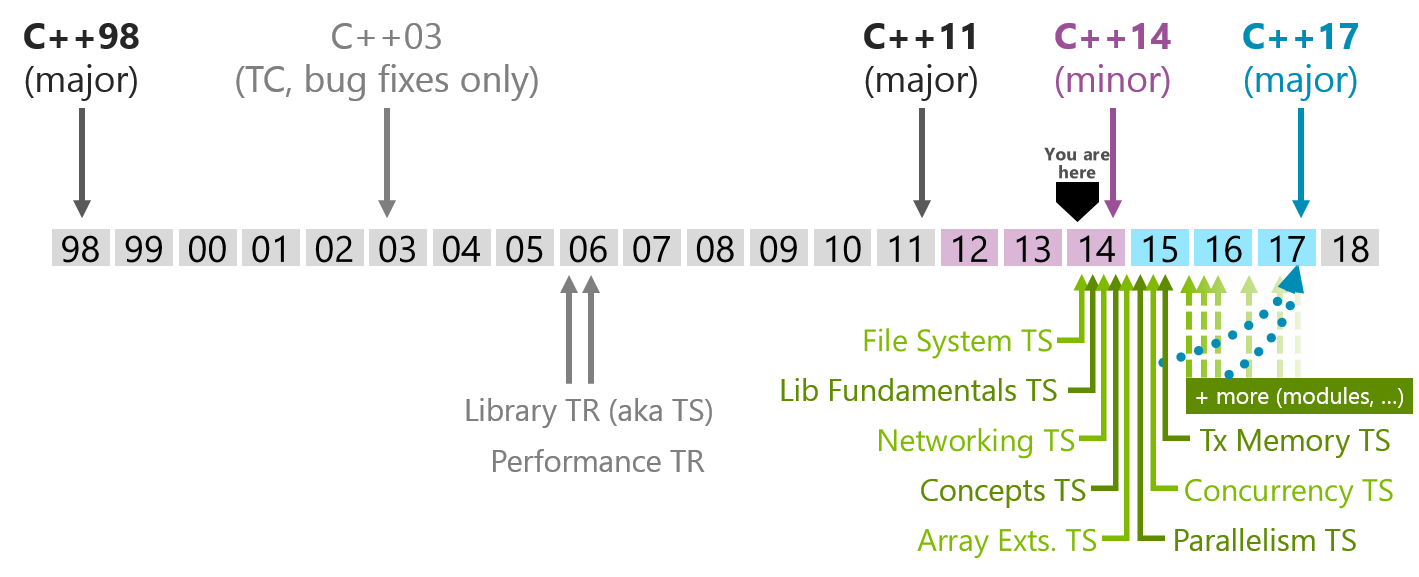
\includegraphics[scale=0.6]{imagens/evolucaoCpp.png}
	\caption{Linha do tempo: evolu��o da especifica��o da linguagem C++}
	\label{fig:evolucaoCpp}
\end{figure}

Muitos recursos adicionados na linguagem pelas especifica��es C++11 e C++14 foram utilizados no desenvolvimento deste trabalho. Nas se��es seguintes ser�o descritos alguns destes recursos, e como eles contribuem para melhorar algumas limita��es que eram impostas pela linguagem.

\subsubsection{Listas de Inicializa��o}
\label{sec:listasInicializacao}

Um recurso simples e ao mesmo tempo bastante �til, as \textbf{listas de inicializa��o} foram criadas com o objetivo de facilitar a instancia��o de estruturas do tipo \textit{container} (lista, pilha, fila, tabelas \textit{hash}, etc) com um conjunto de elementos adicionados. � importante ressaltar que a linguagem na especifica��o C++98 j� permitia a inicializa��o de vetores com uma lista de elementos \cite{professionalCpp}.

Este recurso se baseia na utiliza��o de uma nova classe chamada \textit{\textbf{``initializer\_list''}} definida dentro do \textit{namespace}\footnote{Mecanismo presente na linguagem C++ que permite agrupar estruturas dentro de um espa�o de resolu��o de nomes comum. � utilizado para evitar conflitos de nomes entre estruturas.} ``\textit{std}''. Esta classe implementa um \textit{container} de dados simples, que suporta o acesso aos seus elementos atrav�s do uso de \textbf{iteradores}.  Quando o compilador encontra algum trecho de c�digo com o padr�o ``\{x, y, z\}'' onde ``x'', ``y'' e ``z'' s�o valores literais ou vari�veis que podem ser convertidas para um tipo de dado ``T'' comum de forma impl�cita, ele constr�i um objeto do tipo ``\textit{initializer\_list<T>}''. Sendo assim, para que um objeto possa ser constru�do com uma lista de inicializa��o, basta que sua classe contenha um construtor que recebe como par�metro um objeto do tipo ``\textit{initializer\_list<T>}'' \cite{cppAnnotations}.

No trecho de c�digo \ref{lst:initializerListExample} � demonstrado a utiliza��o das listas de inicializa��o. Primeiramente temos a inicializa��o de um vetor de n�meros inteiros (linha 2) utilizando a sintaxe j� suportada pela linguagem na especifica��o C++98. Em seguida temos a inicializa��o de um objeto do tipo \textit{\textbf{vector\footnote{Classe presente na biblioteca padr�o de C++, e que implementa uma estrutura de lista de elementos utilizando �reas de mem�ria cont�guas.}}} (linha 4) utilizando o novo recurso adicionado na especifica��o C++11. Por �ltimo, temos a defini��o de uma classe projetada para suportar o recurso de listas de inicializa��o (linhas 7 a 9) e em seguida a inicializa��o de um objeto desta classe (linha 13).

\begin{algorithm}
\caption{Inicializa��o de vetores e estruturas \textit{container}}
\label{lst:initializerListExample}
\lstinputlisting[]{codigos/initializerListExample.cpp}
\end{algorithm}

\subsubsection{Navega��o em Grupos de Elementos}
\label{sec:forRangeBasedLoop}

Quando precisamos acessar sequencialmente os elementos de um vetor ou de alguma estrutura do tipo \textit{container} utilizando a linguagem C++, temos basicamente duas op��es: 

\begin{description}
\item[1)Acesso sequencial via �ndice:]
Utilizamos um la�o de repeti��o para gerar valores num�ricos sequenciais dentro do intervalo de posi��es ou �ndices dos elementos que desejamos acessar na estrutura. De posse dos �ndices, podemos acessar os elementos utilizando a sintaxe ``estrutura[�ndice]''. Esta t�cnica pode ser utilizada em vetores e em estruturas \textit{container} que implementam o operador ``[]'' \cite{professionalCpp}. Um exemplo da utiliza��o desta t�cnica � apresentado no trecho de c�digo \ref{lst:acessoSeqIndice}.

\begin{algorithm}
	\caption{Acesso sequencial via �ndice}
	\label{lst:acessoSeqIndice}
	\lstinputlisting[]{codigos/acessoSeqIndiceExample.cpp}
\end{algorithm}

\item[2)Acesso sequencial via iteradores:]
As estruturas \textit{container} presentes na linguagem C++ disponibilizam o acesso a um ponteiro especial que permite navegar entre os elementos que ele cont�m. Estes ponteiros s�o chamados de \textbf{iteradores} e podem ser de dois tipos: constantes e n�o constantes. Os iteradores constantes permitem acessar os elementos em modo somente leitura. Enquanto os n�o constantes permitem a modifica��o dos valores destes elementos \cite{professionalCpp}. Um exemplo da utiliza��o desta t�cnica � apresentado no trecho de c�digo \ref{lst:acessoSeqIterador}.

\begin{algorithm}
	\caption{Acesso sequencial via iteradores}
	\label{lst:acessoSeqIterador}
	\lstinputlisting[]{codigos/acessoSeqIteradorExample.cpp}
\end{algorithm}
\end{description}

Na especifica��o C++11 foi adicionada uma varia��o do la�o de repeti��o \textit{\textbf{``for''}} que � basicamente uma simplifica��o das t�cnicas 1 e 2 descritas anteriormente. Considerando que temos um grupo de elementos do tipo ``T'' armazenados em uma estrutura (vetor ou \textit{container}) com uma inst�ncia chamada ``elementos'', podemos navegar sobre os elementos desta inst�ncia utilizando um trecho de c�digo no formato ``for (T e : elementos) \{...\}''. Neste caso, o c�digo contido entre as chaves ser� executado uma vez para cada elemento contido em ``elementos'', onde a vari�vel ``e'' assume o valor de cada um destes elementos \cite{professionalCpp}.

Esta nova varia��o pode ser utilizada tanto com vetores quanto com estruturas do tipo \textit{container}, e tamb�m � poss�vel navegar sobre os elementos em modo somente leitura. No trecho de c�digo \ref{lst:forNovaSintaxe} � demonstrada a utiliza��o desta nova sintaxe de diferentes formas.

\begin{algorithm}
	\caption{Acesso sequencial com nova sintaxe (C++11)}
	\label{lst:forNovaSintaxe}
	\lstinputlisting[]{codigos/forNovaSintaxe.cpp}
\end{algorithm}

\subsubsection{Novo Identificador para Ponteiros Nulos}
\label{sec:nullptr}

A linguagem C++ permite a manipula��o direta de mem�ria a partir da utiliza��o de \textbf{ponteiros}, vari�veis estas que armazenam o endere�o inicial da por��o de mem�ria em que uma estrutura de dados est� sendo armazenada durante a execu��o de um programa \cite{professionalCpp}. 

A manipula��o de ponteiros � uma tarefa complexa, que deve ser feita com muito cuidado. Uma tentativa de acesso a uma regi�o de mem�ria inv�lida pode gerar problemas graves durante a execu��o do programa. Para evitar este tipo de problema, uma boa pr�tica consiste em invalidar ou anular ponteiros durante a sua inicializa��o e quando o seu uso chegou ao fim (o que acontece por exemplo quando desalocamos a regi�o de mem�ria apontada por ele) \cite{professionalCpp}.

Para anular um ponteiro simplesmente atribu�mos a ele o valor 0. Por�m, na maioria dos ambientes de desenvolvimento, temos a presen�a de uma macro chamada ``NULL'' que � utilizada no local do valor 0 durante a anula��o de um ponteiro para fins de legibilidade. 

Esta metodologia pode levar a comportamentos inesperados do c�digo durante a execu��o, visto que a macro � expandida para o valor inteiro 0 durante a compila��o. Se temos duas fun��es com o mesmo nome, onde uma recebe um ponteiro como par�metro e a outra recebe um n�mero inteiro, ao executar esta fun��o passando a macro ``NULL'', a vers�o que recebe o n�mero inteiro ser� executada, gerando assim um comportamento inesperado. 

Com o objetivo de resolver este problema a especifica��o C++11 prev� a exist�ncia do identificador \textbf{``nullptr''} para ser utilizado com o significado de ponteiro nulo. Ent�o se no mesmo problema citado execut�ssemos a fun��o passando ``nullptr'' como par�metro, a vers�o que recebe o ponteiro ser� executada \cite{professionalCpp}. O exemplo citado pode ser observado no trecho de c�digo \ref{lst:nullptr}.

\begin{algorithm}
	\caption{Novo identificador para ponteiros nulos}
	\label{lst:nullptr}
	\lstinputlisting[]{codigos/nullptr.cpp}
\end{algorithm}

\subsubsection{Infer�ncia de Tipos}
\label{sec:inferenciaTipos}

A linguagem C++ � uma linguagem de tipagem est�tica, ou seja, todas as vari�veis declaradas no c�digo devem ter seu tipo de dado especificado em momento de compila��o \cite{cppAnnotations}. Esta caracter�stica acaba em certas situa��es deixando o c�digo de declara��o de vari�veis muito grande. Veja por exemplo o trecho de c�digo \ref{lst:declaracaoGrande}, onde s�o declarados um \textit{container} para uma lista de inteiros e um iterador para esta lista.

\begin{algorithm}
	\caption{Trecho de declara��o longo}
	\label{lst:declaracaoGrande}
	\lstinputlisting[]{codigos/declaracaoLonga.cpp}
\end{algorithm}

Com a finalidade de reduzir estes trechos de c�digo, a especifica��o C++11 introduziu um mecanismo de infer�ncia ou detec��o autom�tica de tipos de vari�veis atrav�s do uso das palavras-chave \textbf{``auto''} e \textbf{``decltype''} \cite{professionalCpp}. 

A primeira � utilizada durante a atribui��o de valores que j� tem um tipo de dado definido por outro mecanismo, como por exemplo, pelo retorno de uma fun��o ou pelo uso do operador de instancia��o \textit{\textbf{``new''}}. O trecho de c�digo \ref{lst:declaracaoGrande} poderia ser simplificado para o c�digo em \ref{lst:declaracaoPequena}.

\begin{algorithm}
	\caption{Trecho de declara��o curto usando \textbf{``auto''}}
	\label{lst:declaracaoPequena}
	\lstinputlisting[]{codigos/declaracaoCurta.cpp}
\end{algorithm}

O uso da palavra-chave ``auto'' tem uma particularidade importante que deve ser levada em considera��o durante o seu uso. O tipo deduzido � o resultado do tipo do valor atribu�do � vari�vel ap�s a remo��o do modificador \textbf{``const''}\footnote{Utilizado para declarar vari�veis constantes, ou seja, que n�o podem ser usadas para modificar valores.} e do modificador \textbf{``\&''}\footnote{Neste contexto se refere ao modificador para declara��o de vari�veis do tipo refer�ncia na linguagem C++.} \cite{professionalCpp}. Esta particularidade pode levar a resultados inesperados, como o que pode ser observado no trecho de c�digo \ref{lst:autoParticularidade} na linha 10, onde a dedu��o de tipo ir� levar a cria��o de uma vari�vel do tipo inteiro com o valor copiado do retorno da fun��o ``constRef'', enquanto que o valor atribu�do originalmente � de uma refer�ncia para um valor inteiro constante.

\begin{algorithm}
	\caption{Particularidade do uso da palavra-chave \textbf{``auto''}}
	\label{lst:autoParticularidade}
	\lstinputlisting[]{codigos/autoParticularidade.cpp}
\end{algorithm}

Nestas situa��es podemos utilizar a palavra-chave ``decltype'' para alcan�ar o comportamento requerido. A fun��o desta palavra-chave � avaliar o tipo de dado do resultado de uma express�o qualquer \cite{professionalCpp}. Ela pode ser utilizada em qualquer lugar do c�digo onde se espera a especifica��o de um tipo de dado, como por exemplo em declara��es de vari�veis e como par�metros para estruturas gen�ricas (que utilizam o mecanismo de \textbf{``templates''}\footnote{Mecanismo presente na linguagem C++ que permite o desenvolvimento de c�digo que pode trabalhar com diferentes tipos de dados. � muito utilizado na constru��o de estruturas do tipo \textit{container}.}). 

No trecho de c�digo \ref{lst:decltype} podemos ver a utiliza��o desta palavra-chave. Neste caso a vari�vel ``numero'' (linha 10) ir� ser deduzida como uma refer�ncia para um valor inteiro constante, que � exatamente o tipo retornado pela fun��o ``constRef''. Por�m o c�digo gerado para a dedu��o n�o � t�o simplificado, o que levou a proposta da adi��o da constru��o \textbf{``decltype(auto)''} (linha 12) pela especifica��o C++14, que tem o mesmo resultado neste caso \cite{professionalCpp}.

\begin{algorithm}
	\caption{Dedu��o de tipo com o uso da palavra-chave \textbf{``decltype''}}
	\label{lst:decltype}
	\lstinputlisting[]{codigos/decltype.cpp}
\end{algorithm}

\subsubsection{Programa��o Funcional}
\label{sec:programacaoFuncional}

O conceito de programa��o funcional prop�e que fun��es e m�todos sejam tratados de forma igualit�ria com vari�veis e objetos, no aspecto de poderem ser transportados entre contextos de execu��o, ser armazenados em estruturas espec�ficas, ser criados sob demanda e ser utilizados como par�metros para outras fun��es e/ou m�todos \cite{fastDelegates}.

A maneira tradicional utilizada para manipular fun��es e m�todos na linguagem C++ consiste do uso de ponteiros. Por�m esta metodologia utiliza uma sintaxe bem dif�cil e existem v�rios problemas ou limitadores em rela��o � convers�o destes ponteiros. Um grande problema encontrado � que ponteiros para fun��es (declaradas no contexto global) e m�todos (declarados dentro de classes, exceto os est�ticos neste caso) possuem sintaxe de declara��o diferentes e n�o s�o convert�veis entre si \cite{fastDelegates}.

No trecho de c�digo \ref{lst:ponteiroFuncoesMetodos} � demonstrada a sintaxe do uso de ponteiros para fun��es e m�todos. Na linha 16 � declarado um ponteiro para a fun��o ``getTexto'', e na linha 18 � declarado um para o m�todo de mesmo nome presente na classe ``Exemplo''. Note que apesar da fun��o e do m�todo possu�rem o mesmo prot�tipo (tipo de retorno e par�metro) a sintaxe para declara��o de seus ponteiros � diferente e eles n�o podem ser convertidos entre si.

\begin{algorithm}
	\caption{Sintaxe para utiliza��o de ponteiros para fun��es e m�todos}
	\label{lst:ponteiroFuncoesMetodos}
	\lstinputlisting[]{codigos/ponteiroFuncoesMetodos.cpp}
\end{algorithm}

A especifica��o C++11 prop�e a unifica��o da representa��o destes ponteiros como inst�ncias da classe \textbf{``function''} que � definida dentro do \textit{namespace} ``std''. Esta classe consegue representar ponteiros para fun��es, m�todos e refer�ncias para \textit{\textit{``function objects''}}\footnote{Inst�ncias de classes que reimplementam a fun��o do operador par�nteses.} \cite{professionalCpp}.

O trecho de c�digo \ref{lst:ponteiroFuncoesMetodos} pode ser reescrito com o uso desta classe conforme o exemplo \ref{lst:stdFunction}. Note que para atribuir um ponteiro para m�todo � preciso utilizar a fun��o \textbf{``bind''} para associar um objeto com o m�todo a ser apontado (linha 22). Com esta nova sintaxe apontadores para m�todos e fun��es com o mesmo prot�tipo podem ser convertidos entre si.

\begin{algorithm}
	\caption{Unifica��o da representa��o de ponteiros para m�todos e fun��es}
	\label{lst:stdFunction}
	\lstinputlisting[]{codigos/stdFunction.cpp}
\end{algorithm}

Outra funcionalidade adicionada pela especifica��o C++11 foi o suporte a defini��o de m�todos an�nimos, tamb�m conhecidos como \textbf{express�es lambda}. Esta funcionalidade consiste na capacidade de criar fun��es sob demanda durante blocos de execu��o do programa. Express�es lambda tamb�m podem ser armazenadas em inst�ncias da classe \textit{``function''} \cite{professionalCpp}. 

\begin{figure}[!htb]
\centering
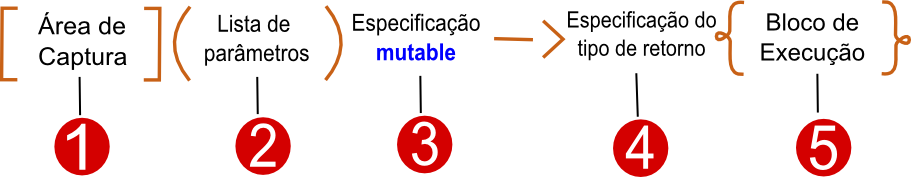
\includegraphics{imagens/LambdaExpression.png}
\caption{Sintaxe b�sica das express�es lambda}
\label{fig:lambdaExpression}
\end{figure}

A sintaxe b�sica para utiliza��o de express�es lambda � demonstrada na imagem \ref{fig:lambdaExpression}. Os blocos presentes nesta constru��o s�o explicados em seguida:

\begin{description}
\item[1) �rea de captura (\textit{Capture specification}):]
As express�es lambda podem capturar as vari�veis presentes no contexto atual de execu��o para utilizar seus valores no seu bloco de execu��o. Esta captura pode feita por valor, onde � efetuado uma c�pia dos valores das vari�veis do contexto alvo, ou pode ser feita por refer�ncia, onde as vari�veis ser�o referenciadas no bloco de execu��o da express�o, ou seja, podemos trabalhar com modifica��o de valores das vari�veis originais. 
Neste �ltimo caso � importante garantir que as vari�veis capturadas existem no momento de execu��o da express�o, caso contr�rio teremos uma exce��o de acesso a posi��o inv�lida de mem�ria. A captura pode ser feita especificando cada vari�vel que queremos capturar, como por exemplo no trecho ``[a, \&b]'' capturamos a vari�vel ``a'' por valor e ``b'' por refer�ncia. Ou podemos capturar todas as vari�veis do contexto utilizando ``[=]'' para capturar todas as vari�veis por valor ou ``[\&]'' para capturar por refer�ncia. Caso n�o seja necess�rio capturar vari�veis especificamos atrav�s do de colchetes sem conte�do, assim ``[]'' \cite{cppAnnotations}.

\item[2) Lista de par�metros (\textit{Parameter specification}):]
� onde � especificada a lista de par�metros que a express�o lambda recebe. A sintaxe � a mesma utilizada na defini��o de prot�tipos de fun��es e m�todos. Por exemplo no trecho ``(int a, char b)'' dizemos que a express�o recebe um n�mero inteiro que ser� referenciado no corpo da express�o como ``a'' e tamb�m recebe um caractere que ser� referenciado como ``b'' \cite{cppAnnotations}.

\item[3) \textit{Mutable specification}:]
Por padr�o, vari�veis capturadas por valor s�o tratadas dentro do bloco de execu��o da express�o como do tipo constante, ou seja, n�o podemos modificar seus valores. Caso utilizemos o modificador \textbf{``mutable''} elas n�o ser�o mais tratadas como do tipo constante, ent�o poderemos manipular os valores copiados no bloco de execu��o da express�o \cite{cppAnnotations}.

\item[4) Especifica��o do tipo de retorno (\textit{Return type specification}):]
Neste ponto devemos especificar o tipo de dado que ser� retornado pela express�o lambda. Caso a express�o n�o retorne valores ou o tipo do valor retornado pode ser deduzido pelo compilador, podemos omitir esta parte \cite{cppAnnotations}.

\item[5) Bloco de execu��o (\textit{Lambda body}):]
Consiste do bloco de c�digo que ser� executado quando a express�o for utilizada. Assim como a lista de par�metros, este trecho de defini��o segue a mesma sintaxe da defini��o de fun��es e m�todos comuns. Podem ser utilizadas quaisquer constru��es v�lidas para blocos de execu��o na linguagem C++. � importante ressaltar tamb�m que n�o h� um limite de tamanho para o bloco, por�m express�es lambda geralmente s�o bem concisas e simplificadas, ocupando poucas linhas. Caso a express�o comece a ficar muito grande e complexa, talvez seja melhor definir uma fun��o comum para que possa ser reutilizada por outros componentes do programa \cite{cppAnnotations}.

\end{description}

No trecho de c�digo \ref{lst:lambdaExpression} temos um exemplo de defini��o de uma express�o lambda com o mesmo prot�tipo utilizado nos exemplos anteriores. Note que a express�o pode ser armazenada em uma inst�ncia da classe ``\textit{function}'' e a sua execu��o � feita da mesma maneira que os ponteiros para fun��es e m�todos armazenados nestas inst�ncias.

\begin{algorithm}
	\caption{Exemplo de defini��o de uma express�o lambda}
	\label{lst:lambdaExpression}
	\lstinputlisting[]{codigos/lambdaExpression.cpp}
\end{algorithm}


\subsubsection{Ponteiros Inteligentes (\textit{Smart Pointers})}
\label{sec:ponteirosInteligentes}

Um dos maiores desafios enfrentados por desenvolvedores que utilizam a linguagem C++ consiste na garantia da libera��o de blocos de mem�ria alocados dinamicamente a partir do uso de ponteiros. Sempre que alocamos uma regi�o de mem�ria a partir do uso do operador \textbf{\textit{``new''}}, temos que garantir que em algum ponto do c�digo aquela regi�o ser� liberada, tarefa que deve ser realizada explicitamente com o uso do operador \textbf{\textit{``delete''}} \cite{cppAnnotations}.

Regi�es de mem�ria alocada que n�o s�o liberadas, ir�o persistir marcadas como utilizadas durante todo o fluxo de execu��o do programa, causando assim um efeito de utiliza��o extra de mem�ria indevida tamb�m conhecido como \textbf{\textit{``memory leak''}} \cite{professionalCpp}. 

Com o objetivo de evitar este tipo de problema, a especifica��o C++11 prev� a cria��o de ponteiros inteligentes ou \textit{``smart pointers''}, que s�o basicamente estruturas que simulam o funcionamento de um ponteiro comum, por�m adicionando mecanismos de gerenciamento de mem�ria. Do ponto de vista de padr�es de projeto, um \textit{smart pointer} seria um \textit{proxy} para a interface de ponteiros comuns \cite{cppAnnotations}.

A especifica��o C++11 define a presen�a de tr�s \textit{smart pointers}, sendo eles:

\begin{description}
	\item[1) \textbf{\textit{``unique\_ptr''}}:]
	Este ponteiro t�m basicamente as mesmas caracter�sticas de um ponteiro comum. A �nica diferen�a � que ele automaticamente libera a regi�o de mem�ria apontada por ele quando ele � deletado ou quando o escopo de sua utiliza��o chega ao fim \cite{professionalCpp}.
	\item[2) \textbf{\textit{``shared\_ptr''}}:]
	Este ponteiro possui uma funcionalidade um pouco mais avan�ada. Ele mant�m um contador interno que armazena a quantidade de refer�ncias que existem para a regi�o de mem�ria apontada por ele, ou seja, ele armazena quantas inst�ncias do tipo ``shared\_ptr'' se encontram ativas no momento para aquela regi�o de mem�ria. O contador � incrementado quando o ponteiro � copiado e decrementado quando inst�ncias de ponteiros s�o deletadas ou perdem escopo. Somente quando o contador chegar a zero, ou seja, quando n�o existir mais nenhuma c�pia do ponteiro original ativa, a regi�o de mem�ria ser� automaticamente liberada \cite{professionalCpp}.
	\item[3) \textbf{\textit{``weak\_ptr''}}:]
	Este ponteiro � utilizado para testar se uma inst�ncia de ``shared\_ptr'' ainda � v�lida (ainda n�o foi desalocada), e caso o for, permite efetuar uma c�pia desta inst�ncia para acessar a regi�o de mem�ria apontada \cite{professionalCpp}.
\end{description}

O trecho de c�digo \ref{lst:smartPointer} demonstra a utiliza��o dos tr�s tipos de \textit{smart pointers} descritos anteriormente. Nele s�o alocados dois espa�os de mem�ria para armazenar dados do tipo inteiro dentro de um escopo de execu��o delimitado por chaves. Assim que o escopo � finalizado, ambos os ponteiros desalocam a regi�o de mem�ria apontada por eles automaticamente. No c�digo tamb�m � mostrado como utilizar um ``weak\_ptr'' para verificar se um ``shared\_ptr'' ainda � v�lido a partir da utiliza��o do m�todo \textbf{``lock''} que retorna uma c�pia deste segundo ponteiro no caso de valida��o ou retorna ``nullptr'' caso contr�rio.

\begin{algorithm}
	\caption{Utilizando \textit{smart pointers}}
	\label{lst:smartPointer}
	\lstinputlisting[]{codigos/smartPointers.cpp}
\end{algorithm}

\section{O \textit{Framework} Qt}
\label{sec:qt}
Qt � um \textit{framework} multiplataforma voltado para a cria��o de aplicativos com interface gr�fica utilizando a linguagem C++. Sua primeira vers�o foi lan�ada em 1995 pelos seus criadores \textit{Haavard Nord} e \textit{Eirik Chambe-Eng} em sua empresa chamada \textit{Trolltech} \cite{qtGuiProgramming}.

O objetivo do \textit{framework} � basicamente prover uma interface de programa��o padr�o para executar tarefas como cria��o de interface gr�fica, programa��o paralela e acesso a banco de dados, para todas as plataformas suportadas. Esse comportamento � alcan�ado atrav�s do direcionamento da execu��o das tarefas para implementa��es espec�ficas existentes na plataforma alvo \cite{qtGuiProgramming}. Uma caracter�stica interessante do \textit{framework} � a adapta��o da interface gr�fica criada ao seu ambiente de execu��o. Uma janela executada em um sistema operacional suportado assume a apar�ncia nativa do mesmo, como � poss�vel verificar nas figuras \ref{fig:windowLinux}, \ref{fig:windowWindows} e \ref{fig:windowMac}, onde temos uma janela de um programa sendo exibida nos tr�s sistemas suportados da plataforma \textit{desktop}.

\begin{figure}[!htb]
\centering
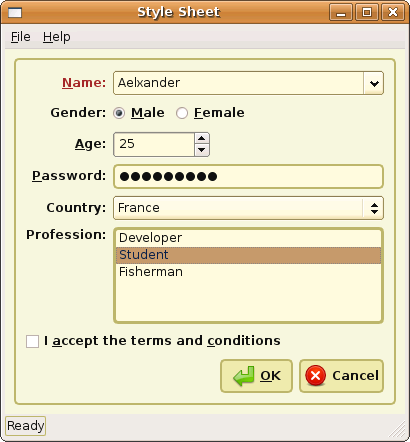
\includegraphics{imagens/windowLinux.png}
\caption{Janela no GNU/Linux}
\label{fig:windowLinux}
\end{figure}
\begin{figure}[!htb]
\centering
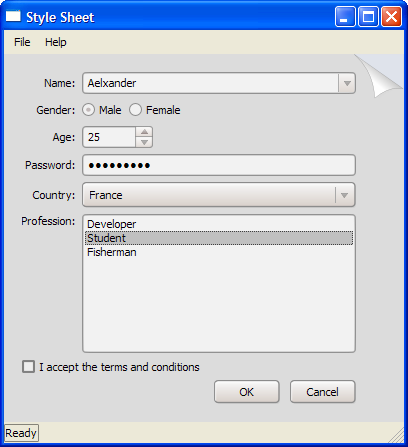
\includegraphics[scale=0.8]{imagens/windowWindows.png}
\caption{Janela no Microsoft Windows XP}
\label{fig:windowWindows}
\end{figure}
\begin{figure}[!htb]
\centering
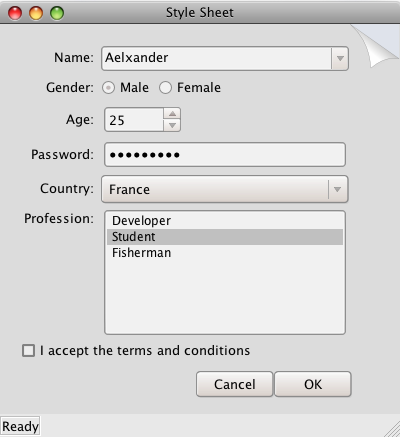
\includegraphics[scale=0.8]{imagens/windowMac.png}
\caption{Janela no Mac Os}
\label{fig:windowMac}
\end{figure}

Inicialmente o \textit{framework} era totalmente focado na padroniza��o do processo de cria��o de interface gr�fica entre diferentes plataformas, por�m ao longo de sua exist�ncia foram sendo adicionadas novas fun��es voltadas para tarefas rotineiras no desenvolvimento de \textit{software}, como por exemplo acesso a banco de dados, programa��o paralela e manipula��o de arquivos multim�dia (v�deos e imagens). Com a adi��o destes novos componentes, o \textit{framework} acabou crescendo muito, o que levou aos desenvolvedores o reestruturarem em forma de m�dulos de forma que o desenvolvedor possa adicionar em seu projeto somente os m�dulos que pretende utilizar, diminuindo o tamanho final do execut�vel gerado para distribui��o de seu aplicativo \cite{qtGuiProgramming}.

Neste trabalho s�o utilizados basicamente tr�s dos m�dulos existentes no \textit{framework}, sendo eles o \textbf{QtSql}, o \textbf{QtTest} e o \textbf{QtCore}. O QtSql � um m�dulo voltado para utiliza��o de \textbf{Sistemas Gerenciadores de Bancos de Dados Relacionais} (ver se��o \ref{sec:sgbd}) como forma de persist�ncia dos dados gerados pelo aplicativo. Ele prov� suporte para utiliza��o dos sistemas mais populares, como \textbf{MySQL}, \textbf{Oracle}, \textbf{PostgreSQL},
\textbf{Sybase}, \textbf{DB2}, \textbf{SQLite}, \textbf{Interbase} e \textbf{ODBC} \cite{qtFoundations}. Esse m�dulo ser� utilizado como apoio para utiliza��o de bancos de dados relacionais nas plataformas \textbf{Microsoft Windows} e \textbf{GNU/Linux}. 

O QtTest � um m�dulo voltado para a cria��o de testes unit�rios. Os testes s�o utilizados para validar o funcionamento do \textit{software} desenvolvido ao longo de sua exist�ncia. Geralmente s�o executados quando � feita alguma modifica��o no c�digo, como por exemplo adi��o de novos componentes. E, por fim, QtCore � o m�dulo principal do \textit{framework}. Ele � respons�vel por prover rotinas para programa��o paralela, convers�o de tipos, al�m de adicionar tipos de dados muito importantes na utiliza��o de bancos de dados, como o \textbf{\textit{QDateTime}}\footnote{Tipo de dado que armazena um valor de data e hora. N�o existe um tipo de dado nativo em C++ para esta finalidade.} \cite{qtFoundations}. 

No momento da cria��o deste documento, o framework est� em sua vers�o 5.3 (vers�o que � utilizada no trabalho), e � compat�vel com os sistemas operacionais \textit{GNU/Linux}, \textit{Microsoft Windows} e \textit{Mac OS} na plataforma \textit{desktop}. Ele oferece tamb�m suporte a dispositivos embarcados com sistema operacional \textit{GNU/Linux} e para dispositivos m�veis com os sistemas \textit{Android}, \textit{IOS} e \textit{Windows Phone}.

\section {Sistemas Gerenciadores de Bancos de Dados Relacionais}
\label{sec:sgbd}

Assim como as linguagens orientadas a objetos s�o consideradas um padr�o para desenvolvimento de \textit{software}, os Sistemas Gerenciadores de Bancos de Dados Relacionais ou \textbf{SGBD}s s�o considerados um padr�o para armazenamento estruturado de informa��es \cite{ormPaper}.

Os SGBDs utilizam um modelo de persist�ncia denominado \textbf{modelo relacional}, que se baseia no uso de \textbf{tabelas} e \textbf{colunas}. As tabelas representam entidades, ou um grupo de informa��o a ser armazenado, e podem se relacionar com outras tabelas para promover regras de armazenamento. As colunas representam as caracter�sticas da entidade armazenada. Neste modelo, quando armazenamos um registro, ele � acrescentado como uma linha em uma ou mais tabelas relacionadas. Nas tabelas, pode ser aplicado o conceito de unicidade dos registros armazenados, atrav�s da defini��o de um conjunto de colunas que deve representar uma combina��o de valores �nica dentre os registros armazenados. Este conjunto de colunas define o que chamamos de \textbf{chave prim�ria} da tabela ou, em ingl�s,  
\textbf{\textit{``primary key''}} \cite{ormPaper}.

A defini��o de chaves prim�rias nas tabelas criadas permite a cria��o de rela��es entre elas atrav�s do uso de refer�ncias entre suas chaves. A refer�ncia em uma tabela para uma chave prim�ria de outra tabela � conhecida como \textbf{chave estrangeira} ou, em ingl�s, \textbf{\textit{``foreign key''}} \cite{ormPaper}. Na figura \ref{fig:modeloRelacional} temos um exemplo de defini��o de duas tabelas, uma representando registros de pessoas e outra de telefones. Elas est�o relacionadas, de modo que um registro de telefone pertence a uma pessoa. Este comportamento � obtido atrav�s da defini��o da chave estrangeira ``TelefoneId'' na tabela ``Pessoa'', que se refere � chave ``Id'' na tabela ``Telefone''.

\begin{figure}[!htb]
\centering
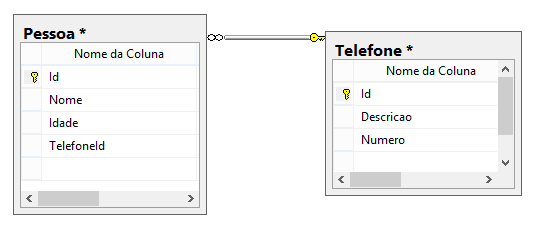
\includegraphics{imagens/modeloRelacional.png}
\caption{Exemplo de defini��o de tabelas e rela��es}
\label{fig:modeloRelacional}
\end{figure}

Uma das funcionalidades mais importantes apresentada pelos SGBDs � a capacidade de aplica��o de rotinas complexas de pesquisa usando a linguagem \textbf{SQL}. Esta linguagem define um conjunto de opera��es que permite executar inser��es, modifica��es, remo��o e busca de registros armazenados em um SGBD \cite{ormPaper}. Talvez esta funcionalidade seja a causa de sua grande utiliza��o e aceita��o. Neste trabalho � utilizado o SGBD \textbf{PostgreSQL} (ver se��o \ref{sec:postgresql}).

\section{O PostgreSQL}
\label{sec:postgresql}
O PostgreSQL � um SGBD de c�digo aberto, e com licen�a de uso gratuita para qualquer pessoa sobre qualquer prop�sito. Ele pode ser utilizado, modificado e redistribu�do livremente. Este SGBD � derivado do projeto \textbf{POSTGRES} desenvolvido na Universidade de Berkeley na Calif�rnia no ano de 1986. Por ser um \textit{software} de c�digo aberto desenvolvido em comunidade, ele � conhecido por ser pioneiro na adi��o de novas funcionalidades, e se mant�m sempre atualizado em rela��o aos conceitos e especifica��es da linguagem SQL \cite{postgresqlDoc}.


\section{A combina��o de SGBDs com Linguagens Orientadas a Objetos}
\label{sec:sgbdWithOop}

A princ�pio, os programas trabalham com dados em mem�ria principal, que � vol�til. Isto �, ao desligarmos o equipamento todos os dados s�o perdidos. Devido a isso,  necessitamos de algum mecanismo de persist�ncia, ou seja, que permita a grava��o de dados importantes em mem�ria secund�ria, n�o vol�til \cite{ormPaper}. 

A combina��o mais comumente utilizada para alcan�ar este cen�rio � o uso de linguagens orientadas a objetos para desenvolver o \textit{software} e o uso de SGBDs para armazenar os dados gerados pelo \textit{software} \cite{hibernateInAction}. Por�m, os dados no contexto orientado a objetos e no contexto relacional s�o estruturados de maneiras diferentes, portanto precisamos realizar uma convers�o ou mapeamento dos dados durante a transi��o de contextos.

Quando estamos trabalhando com classes simples (n�o compostas por membros de outras classes), o mapeamento segue uma l�gica simples. Podemos criar uma correspond�ncia entre a classe e sua respectiva tabela, onde os atributos da classe s�o mapeados para colunas de uma tabela. Por�m quando come�amos a utilizar mecanismos mais avan�ados da orienta��o a objetos como heran�a e composi��o, o mapeamento entre os contextos se torna mais complexo \cite{ormPaper}.

Mesmo quando temos um cen�rio onde o mapeamento � simples, precisamos gerar c�digo de convers�o. As linguagens de programa��o fornecem bibliotecas ou \textbf{\textit{APIs}}\footnote{\textit{Application Programming Interface}. Define uma interface de um conjunto de bibliotecas de \textit{software}.} que permitem a comunica��o com SGBDs atrav�s do envio de comandos em linguagem SQL \cite{ormPaper}. O c�digo gerado para executar a transi��o de dados entre os dois contextos geralmente segue a seguinte sequ�ncia de passos:

\begin{enumerate}
	\item Carregar um \textit{driver} de comunica��o com o SGBD utilizado e abrir a conex�o;
	\item Criar um objeto que permita a montagem de c�digo SQL;
	\item Enviar o comando para o SGBD para que seja executado;
	\item Recuperar e processar os dados ou resposta gerados pelo SGBD;
	\item Liberar os recursos alocados para execu��o da tarefa, como por exemplo fechar a conex�o com SGDB.
\end{enumerate}

No trecho de c�digo \ref{lst:qtsql_mapclasse} temos um esbo�o de como estas etapas s�o realizadas utilizando a linguagem C++ em conjunto com o m�dulo QtSql do framework Qt (ver se��o \ref{sec:qt}) e comunicando com o SGBD PostgreSQL (ver se��o \ref{sec:postgresql}).
\begin{algorithm}
\caption{Exemplo de comunica��o com SGBD utilizando o m�dulo QtSql}
\label{lst:qtsql_mapclasse}
\lstinputlisting[]{codigos/qtsql_mapclasse.cpp}
\end{algorithm}

A utiliza��o deste tipo de c�digo se torna repetitiva, visto que temos que executar estes passos para todas as classes que armazenam dados utilizando SGBDs. Este tipo de comportamento � indesejado, pois diminui a produtividade do desenvolvimento, al�m do fato de que tarefas repetitivas tem grande potencial de gerarem erros. Outro grande problema que encontramos � que os comandos em linguagem SQL variam entre os SGBDs, portanto ao mudar o SGBD utilizado pelo programa, temos de reescrever os comandos SQL utilizados. Este � outro fator com grande potencial de gera��o de erros, al�m de diminuir a flexibilidade do \textit{software}, tornando, em alguns casos, invi�vel a mudan�a de SGBD \cite{ormPaper}.

Para otimizar a combina��o do uso de linguagens de programa��o orientadas a objetos em conjunto com SGBDs, surgiu o conceito de \textbf{Biblioteca de Mapeamento Objeto Relacional} ou \textbf{ORM} (\textbf{\textit{Object Relational Mapping}}), assunto abordado na se��o \ref{sec:orm}.

%--- Explicar o que � ORM de maneira simples e direta
\section{Bibliotecas de Mapeamento Objeto Relacional}
\label{sec:orm}

As bibliotecas ORM t�m como objetivo principal automatizar as tarefas relacionadas com a transi��o de informa��es entre os contextos orientado a objetos e relacional. N�o existe um conceito universal que defina quais s�o as funcionalidades que uma biblioteca ORM deve oferecer \cite{ormPaper}, por�m as tr�s funcionalidades mais comumente encontradas s�o:

\begin{description}
\item[1) Defini��o de mapeamento:] 
As bibliotecas ORM permitem a defini��o expl�cita da correspond�ncia entre entidades no contexto orientado a objetos (classes) e entidades no contexto relacional (tabelas). Os mecanismos de defini��o deste mapeamento variam entre as implementa��es;
\item[2) Gera��o de banco de dados:]
As bibliotecas ORM geralmente permitem a gera��o autom�tica do banco de dados equivalente �s estruturas do contexto orientado a objetos;
\item[3) Defini��o de uma API:]
Geralmente as bibliotecas ORM disponibilizam interfaces padronizadas para realiza��o de tarefas que envolvam a transi��o de dados entre os dois contextos. Opera��es como salvar, deletar ou pesquisar registros s�o encapsuladas em classes de prop�sito geral que conseguem trabalhar sobre qualquer entidade mapeada.
\end{description}

Nem todas as bibliotecas existentes oferecem as tr�s funcionalidades descritas, mas o mais comum � encontrar uma combina��o das tr�s. Existem ainda bibliotecas que permitem gerar o c�digo de mapeamento e at� mesmo gerar o c�digo das classes a partir da an�lise de um banco de dados existente. Esta funcionalidade � conhecida como \textbf{Mapeamento Reverso} ou \textbf{Engenharia Reversa} \cite{ormPaper}.

As bibliotecas ORM divergem bastante na forma de implementa��o e funcionalidades disponibilizadas. Isso se deve principalmente ao fato da diverg�ncia de recursos entre as pr�prias linguagens de programa��o em que s�o implementadas. Por�m uma decis�o comum a ser tomada no desenvolvimento de uma biblioteca ORM em qualquer linguagem, � a defini��o do ponto de partida para obten��o das informa��es de mapeamento \cite{ormPaper}. Os paradigmas mais utilizados s�o:

\begin{description}
\item[1) Orientado a metadados:]
Neste paradigma, o desenvolvedor informa a estrutura das entidades envolvidas no \textit{software} que devem ser mapeadas atrav�s de alguma fonte externa, como um arquivo XML. Neste arquivo s�o informados metadados\footnote{Informa��es complementares sobre outro conjunto de dados. Podem ser utilizados, por exemplo, para descrever a estrutura destes.} sobre as entidades nos dois contextos, o que permite a biblioteca ORM criar o c�digo de defini��o das classes e do c�digo de mapeamento. Neste modelo podemos utilizar um banco de dados j� existente, ou a biblioteca ORM pode constru�-lo a partir da an�lise dos metadados. A vantagem deste paradigma � a abstra��o total da gera��o de c�digo de manipula��o do banco de dados. E sua grande desvantagem � a limita��o de edi��o do c�digo gerado pela biblioteca. Os c�digos das classes mapeadas ser�o gerados automaticamente pela biblioteca e n�o poder�o ser editados pelo desenvolvedor \cite{ormPaper}.

\item[2) Orientado � aplica��o:]
Neste paradigma o desenvolvedor deve escrever o c�digo das classes de todo o programa normalmente, por�m sem se preocupar com as opera��es de persist�ncia. Ap�s a defini��o das classes, a biblioteca ORM, atrav�s da an�lise do c�digo e opcionalmente metadados, consegue criar o c�digo de persist�ncia. � poss�vel utilizar um banco de dados existente ou a biblioteca pode constru�-lo. A vantagem deste paradigma � a total abstra��o da gera��o de c�digo de manipula��o do banco de dados, e sua grande desvantagem � a alta complexidade de desenvolver o mecanismo de an�lise do c�digo escrito pelo desenvolvedor para inferir informa��es de mapeamento. A defini��o deste mecanismo pode influenciar bastante no desempenho final da aplica��o que utiliza a biblioteca ORM \cite{ormPaper}.

\item[3) Orientado ao banco de dados:]
Neste paradigma o desenvolvedor deve primeiramente criar o banco de dados. Ent�o a biblioteca ORM auxiliada por metadados consegue gerar o c�digo das classes a serem mapeadas e das opera��es de persist�ncia. A grande desvantagem deste paradigma � a n�o abstra��o do conhecimento de banco de dados, visto que o desenvolvedor deve primeiramente definir a estrutura da base de dados a ser utilizada. Outra desvantagem � o desenvolvedor n�o ter a permiss�o de modificar o c�digo das classes mapeadas pela biblioteca ORM. Sua vantagem consiste no melhor controle da defini��o da estrutura da base de dados sendo utilizada \cite{ormPaper}.
\end{description}

As bibliotecas de mapeamento mais robustas possuem a possibilidade de operar nos tr�s paradigmas citados. Em alguns casos, elas ainda permitem que o desenvolvedor tenha controle dos tr�s componentes principais citados pelos paradigmas, ou seja, o desenvolvedor pode definir o c�digo das classes a serem mapeadas, os metadados e construir o banco de dados a ser utilizado, deixando para a biblioteca ORM somente a tarefa de adicionar o c�digo de persit�ncia \cite{ormPaper}.

Existe ainda o conceito de \textbf{transpar�ncia}, que � aplicado a bibliotecas que utilizam o paradigma orientado � aplica��o. Uma biblioteca ORM � transparente quando n�o requer que classes implementem interfaces, ou sigam um modelo espec�fico de c�digo para serem mapeadas \cite{ormPaper}. Estas bibliotecas seguem a filosofia de que as classes envolvidas no \textit{software} n�o precisam saber como, porque ou quando elas ser�o persistidas, ou seja, elas devem se comportar como ``classes ordin�rias'' ou comuns.

Analisando as principais funcionalidades que as bibliotecas ORM possuem, podemos perceber que elas promovem uma melhoria consider�vel de produtividade (economia de tempo de desenvolvimento) al�m de diminuir a complexidade do desenvolvimento de sistemas que lidam com gerenciamento constante de dados persistidos em bancos de dados relacionais \cite{ormPaper}.




%-------------------------------------------------------------
 \chapter{Trabalhos relacionados}
 \label{cap_terceiro}
 Neste cap�tulo ser� descrito um trabalho correlato, que tamb�m prop�s o desenvolvimento de uma biblioteca ORM para C++ e que � utilizado como base para o desenvolvimento deste trabalho. Tamb�m ser� descrita uma biblioteca ORM presente no mercado, que � bastante utilizada em conjunto com o framework Qt no desenvolvimento de aplicativos comerciais. Esta biblioteca ser� utilizada na realiza��o de testes comparativos ao final do trabalho.

\section{Um framework de mapeamento objeto-relacional com um exemplo em C++}
\label{sec:zhangXiaobing}

Em seu trabalho intitulado "Um framework de mapeamento objeto-relacional com um exemplo em C++", \textit{Zhang Xiaobing} apresenta um modelo para desenvolvimento de uma biblioteca ORM que pode ser utilizado na maioria das linguagens orientadas a objetos. Em seu modelo, ele define padr�es a serem utilizados para resolver problemas como mapeamento de classes simples, heran�a, composi��o, associa��o, e ainda define mecanismos de otimiza��o como cria��o de um cache de objetos resgatados do banco de dados \cite{xiaobingZhang}.

Seu modelo define uma biblioteca ORM que segue o paradigma orientado a aplica��o, onde o desenvolvedor ficar� respons�vel por definir toda a parte do c�digo relacionado a cria��o dos objetos a serem mapeados. Todo objeto a ser mapeado deve herdar de uma classe espec�fica, e o desenvolvedor deve reimplementar determinados m�todos de modo a informar para a biblioteca metadados que definem o mapeamento. Devido a esse comportamento dizemos que a biblioteca n�o � transparente. O modelo ainda define uma arquitetura de desenvolvimento em duas camadas:

\begin{description}
\item[1) Camada de objetos (\textit{\textbf{Object Layer}})]
Camada respons�vel por prover uma interface simples para defini��o de classes a serem mapeadas e seus metadados, al�m de trafegar dados entre os objetos mapeados e a camada de persist�ncia. Esta camada � a �nica acess�vel diretamente pelo desenvolvedor.

\item[2) Camada de persist�ncia (\textit{\textbf{Storage Layer}})]
Camada respons�vel por abstrair a comunica��o com o SGBD, provendo rotinas de persist�ncia, concorr�ncia, recupera��o de erros e execu��es de pesquisas no banco de dados. Esta camada n�o � diretamente acess�vel pelo desenvolvedor.
\end{description}

O modelo definido pode ser aplicado em diversas linguagens pelo fato de n�o se aproveitar de recursos espec�ficos de determinadas linguagens, por�m devido a isso ele exige um trabalho adicional do desenvolvedor ao reimplementar m�todos de diversas interfaces definidas. Em alguns momentos, o desenvolvedor deve explicitamente executar fun��es de consulta e ajuste de valores de atributos em suas classes trocando informa��es com o framework para permitir a execu��o de tarefas no banco de dados \cite{xiaobingZhang}. Isso ocorre devido a biblioteca n�o definir um mecanismo de listagem e acesso �s estruturas internas dos objetos mapeados.

Neste trabalho o modelo de Zhang � utilizado como base para a implementa��o de uma biblioteca ORM para C++, por�m com alguns ajustes como a defini��o de uma interface de anota��es para defini��es de mapeamento, e a capacidade de mapeamento de classes arbitr�rias, sem a necessidade de heran�a de uma classe espec�fica (biblioteca transparente).

\section{QxORM}
\label{sec:qxorm}

A QxORM � uma biblioteca ORM de c�digo aberto desenvolvida para ser utilizada em conjunto com o framework Qt. Ela utiliza v�rios m�dulos do framework para auxiliar as tarefas de mapeamento, como por exemplo o m�dulo QtSql para realizar intera��es com os SGBDs. � uma biblioteca que segue o paradigma orientado a aplica��o, e � transparente, ou seja, permite o mapeamento de classes arbitr�rias. Para mapear uma classe, o desenvolvedor deve inserir algumas marca��es na defini��o da classe, e implementar um m�todo utilizando fun��es espec�ficas para registros de informa��es das classes e atributos a serem mapeados. Portanto, nesta biblioteca tamb�m n�o existe um sistema de anota��es \cite{qxorm}.

Esta biblioteca ser� utilizada durante testes de usabilidade, onde ser� comparado a abordagem de especifica��o de mapeamento dela com a interface de anota��es criada neste trabalho. Al�m de testes de usabilidade, tamb�m ser�o feitos testes de desempenho em rela��o ao uso de mem�ria e tempo de resposta. 

%-------------------------------------------------------------
 \chapter{A biblioteca ORM4Qt}
 \label{cap_quarto}
 Desenvolver aplicativos multiplataforma utilizando a linguagem C++ � uma tarefa muito dif�cil, devido � reduzida biblioteca padr�o da linguagem, e aos diversos componentes espec�ficos desenvolvidos para cada plataforma. Esta complexidade pode ser minimizada a partir do uso de \textit{frameworks} multiplataforma, como o  Qt, para compor nosso ambiente de desenvolvimento. Por�m, em compara��o com ambientes oferecidos por linguagens mais recentes, este apresenta poucos mecanismos de automatiza��o de tarefas diversas, ou os que existem apresentam interfaces complexas para utiliza��o. � o que acontece por exemplo com as bibliotecas de mapeamento objeto relacional ou ORM.

Analisando o ambiente de desenvolvimento oferecido a partir da combina��o da linguagem C++ com o \textit{framework} Qt, encontramos algumas implementa��es de bibliotecas ORM, destacando-se o QxOrm. Estas bibliotecas, devido ao pouco suporte a reflex�o oferecido pela linguagem C++, em sua maioria apresentam interfaces de configura��o complexas. Al�m de usarem mecanismos como heran�a e \textbf{"classes \textit{friend}"}\footnote{Este recurso permite que uma classe ou m�todo global externo acesse os componentes privados de uma classe.} para quebra de encapsulamento das classes a serem mapeadas, o que � indesej�vel por aumentar o n�vel de acoplamento do c�digo.

Neste trabalho � proposto o desenvolvimento de uma biblioteca ORM intitulada ORM4Qt para ser utilizada neste ambiente de desenvolvimento. A biblioteca utilizar� o paradigma orientado a aplica��o e a abordagem transparente para defini��o das classes mapeadas. A interface de configura��o do mapeamento ser� feita atrav�s de um mecanismo de anota��es desenvolvido especificamente para a biblioteca. Para a quebra de encapsulamento das classes ser� utilizada a manipula��o de ponteiros de fun��es atrav�s do uso de estruturas de alto n�vel oferecidos pela linguagem C++. A biblioteca desenvolvida ser� capaz de mapear somente classes simples, ou seja, que cont�m somente atributos escalares e n�o utilize heran�a. Posteriormente, ela poder� ser estendida para suportar o mapeamento de classes que utilizem mecanismos mais avan�ados de orienta��o a objetos.

Das bibliotecas ORM existentes para o cen�rio abordado, a QxOrm � a que mais se aproxima das caracter�sticas citadas, portanto ela ser� utilizada em testes ao final do desenvolvimento. Os testes dever�o comparar a configura��o do ambiente de desenvolvimento para utiliza��o das bibliotecas, a facilidade em utiliza��o dos mecanismos de configura��o de mapeamento e a facilidade em migra��o de c�digo legado.

Nas pr�ximas se��es ser�o detalhados os mecanismos utilizados para o desenvolvimento, bem como a arquitetura utilizada.

\section{Arquitetura em camadas}
\label{sec:layersArch}

O desenvolvimento da biblioteca � estruturado em duas camadas, a camada de Objeto ou \textit{\textbf{"Object Layer"}} e a camada de Armazenamento ou \textit{\textbf{"Storage Layer"}}, seguindo a nomenclatura utilizada no trabalho desenvolvido por \textit{Zhang Xiaobing} \cite{xiaobingZhang}. As duas camadas oferecem interfaces acess�veis diretamente pelo desenvolvedor e cooperam entre si atrav�s de troca de informa��es. 

A camada de Objeto tem como objetivo prover uma interface transparente para o desenvolvedor que permita a configura��o das classes a serem mapeadas e prover uma interface para a camada de Armazenamento que permita o acesso aos metadados bem como � estrutura interna das classes sendo mapeadas. Esta camada � a mais complexa de ser desenvolvida devido ao uso intenso de estruturas de baixo n�vel da linguagem para quebra de encapsulamento e cria��o do mecanismo de anota��es. 

A camada de Armazenamento tem como objetivo prover uma interface para o desenvolvedor que permita executar tarefas relacionadas com a persist�ncia de objetos no banco de dados, al�m de definir uma interface comum de gera��o de c�digo SQL que possa ser implementada para diferentes SGBDs. Inicialmente esta interface ser� implementada para o SGBD PostgreSQL, e utilizar� os mecanismos oferecidos pelo m�dulo QtSql para se comunicar com ele.

Na imagem \ref{fig:camadas} temos uma representa��o de alto n�vel da intera��o entre os m�dulos, o desenvolvedor, o banco de dados e as classes a serem mapeadas durante o funcionamento da biblioteca. Nas pr�ximas se��es as duas camadas ser�o detalhadas juntamente com os mecanismos espec�ficos envolvidos no desenvolvimento de cada uma.

\begin{figure}[!htb]
\centering
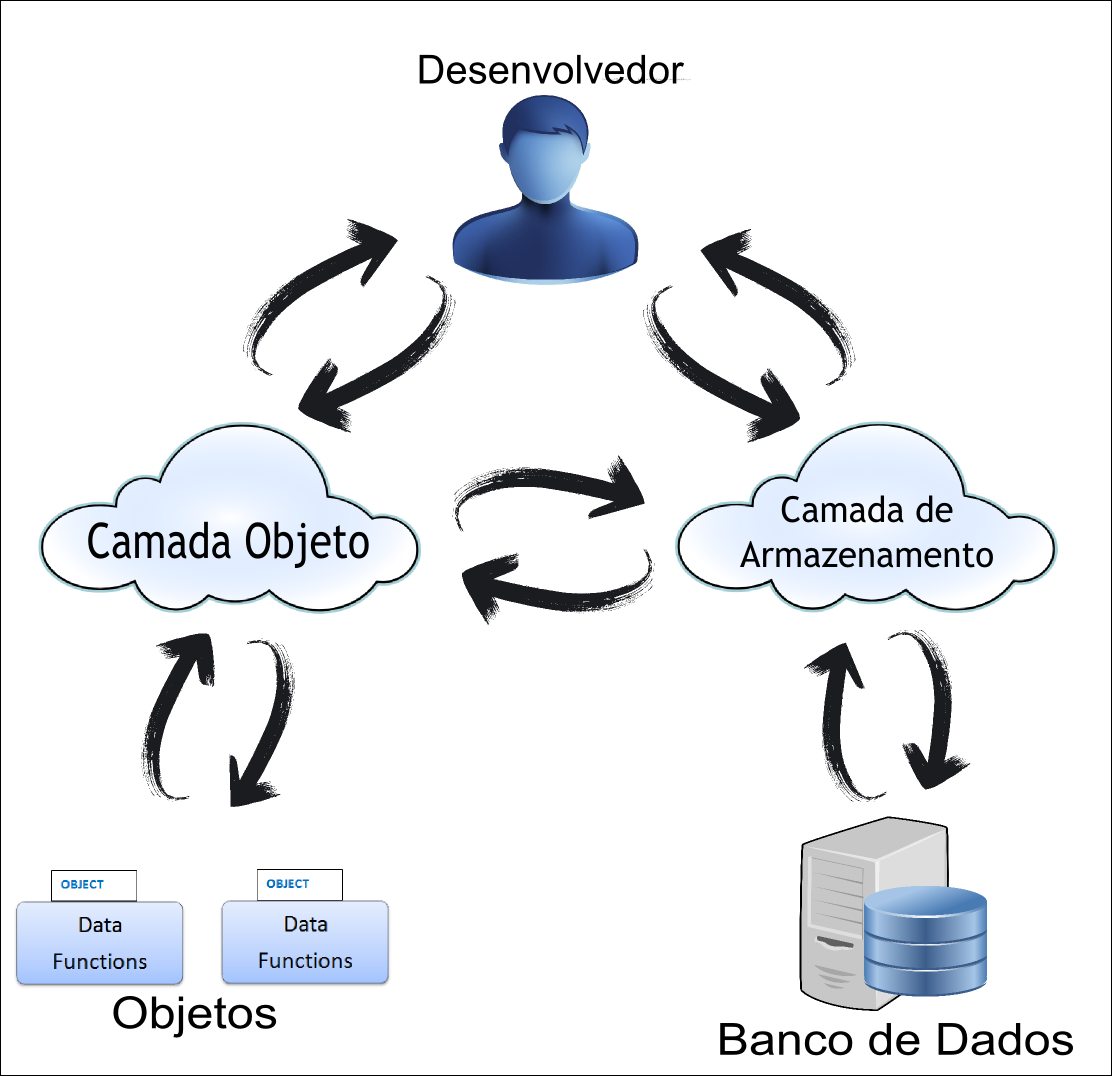
\includegraphics[scale=0.4]{imagens/camadas.png}
\caption{Intera��o entre componentes do software e desenvolvedor}
\label{fig:camadas}

\end{figure}

\section{Camada de Objeto}
\label{sec:objectLayer}

Para que seja poss�vel realizar o mapeamento, a biblioteca ORM deve ser capaz de conhecer e acessar a estrutura interna das classes a serem mapeadas. Existem basicamente dois limitadores que dificultam alcan�ar este cen�rio na linguagem C++. O primeiro deles consiste na possibilidade de o desenvolvedor limitar o acesso � estrutura interna atrav�s das diretivas de prote��o oferecidas pela linguagem durante a defini��o das classes. A biblioteca ORM precisa ter acesso de leitura e escrita nos atributos das classes sendo mapeadas, por�m em geral eles s�o mantidos com permiss�o de acesso privado, onde somente podem ser acessados diretamente de dentro da classe.

O segundo deles � o baixo suporte da linguagem a mecanismos de reflex�o. Antes de acessar os atributos das classes a biblioteca deve saber quais s�o os atributos que a classe cont�m, entretanto em seu atual estado, a linguagem oferece somente informa��es b�sicas sobre os objetos, como por exemplo o nome de sua classe. No trecho de c�digo \ref{lst:reflectionexample} temos um exemplo da obten��o do nome da classe de um objeto em tempo de execu��o. Na linha 1 � criado um objeto da classe Pessoa, e na linha 2 � capturado o nome da classe deste objeto e exibido no console. A sa�da gerada por este programa quando compilado no compilador que acompanha o Visual Studio 2013 � o texto \textit{"class Pessoa"}.

\begin{algorithm}
\caption{Obtendo o nome da classe de um objeto em tempo de execu��o}
\label{lst:reflectionexample}
\lstinputlisting[]{codigos/reflectionExample.cpp}
\end{algorithm}

A camada Objeto utiliza dois mecanismos para contornar estes limitadores, os quais ser�o descritos nas se��es a seguir.

\subsection{Quebrando o encapsulamento das classes}
\label{sec:quebraEncapsulamento}

Quando os atributos das classes s�o declarados com acesso p�blico, a biblioteca ORM pode acess�-los diretamente, por�m este cen�rio n�o � normalmente utilizado pelos desenvolvedores e a utiliza��o da biblioteca impor tal cen�rio � uma caracter�stica indesej�vel e que poderia diminuir sua aceita��o no mercado. Para resolver este problema ent�o partimos do pressuposto de que todos os atributos a serem acessados nas classes a serem mapeadas estar�o com acesso privado, ou seja, s� podem ser acessados de dentro das classes. Com isso em mente podemos tamb�m definir que somente poderemos acessar os atributos das classes atrav�s do uso de um intermediador que componha a estrutura da classe, ou mais precisamente um m�todo que comp�e a interface da classe.

A primeira ideia que vem em mente � utilizar m�todos acessadores (popularmente conhecidos como m�todos \textit{\textbf{"get"}} e \textit{\textbf{"set"}}) criados pelos desenvolvedores, por�m temos alguns limitadores que dificultam a sua utiliza��o. Um deles � que n�o podemos assumir que para todo atributo existem m�todos acessadores, pois podem existir atributos somente leitura ou cujo valor � controlado internamente na classe. Outro limitador � a n�o padroniza��o do prot�tipo dos m�todos acessadores. Estes m�todos podem ser definidos com uma quantidade vari�vel de par�metros, e ainda a linguagem C++ permite a cria��o de varia��es atrav�s da modifica��o do tipo de par�metro e/ou retorno (ponteiro, refer�ncia ou por valor), al�m do uso do modificador \textbf{\textit{"const"}}\footnote{M�todos declarados com este modificador n�o podem modificar o valor dos atributos da classe durante sua execu��o. Esta especifica��o permite ao compilador efetuar otimiza��es no c�digo gerado.} na declara��o de m�todos de leitura.

Devido a estas caracter�sticas, o uso de ponteiros gen�ricos para m�todos, por exemplo, n�o poderia ser utilizado, pois ter�amos que variar a defini��o dos ponteiros de acordo com o prot�tipo dos m�todos utilizados. No trecho de c�digo \ref{lst:prototypeVariant} temos por exemplo as poss�veis varia��es de declara��es de m�todos acessadores para um atributo do tipo inteiro.

\begin{algorithm}
\caption{Exemplo de varia��es na declara��o de m�todos acessadores para atributos tipo inteiro}
\label{lst:prototypeVariant}
\lstinputlisting[]{codigos/prototypeVariant.cpp}
\end{algorithm}

J� que n�o podemos utilizar os m�todos acessadores, a solu��o proposta � a inser��o de m�todos intermediadores na defini��o das classes a serem mapeadas. Dessa maneira podemos criar os m�todos seguindo prot�tipos pr�-definidos, o que nos permite manipul�-los mais facilmente atrav�s de ponteiros. Por�m esta solu��o ainda tem um problema. Se formos criar um m�todo para cada atributo da classe, a quantidade destes pode se tornar muito grande, o que causaria uma modifica��o extrema da interface original da classe mapeada, o que � indesej�vel. Para diminuir os efeitos deste problema � proposto a utiliza��o de \textbf{express�es lambda}.

As express�es lambda s�o estruturas que permitem a cria��o de m�todos an�nimos, ou seja, que n�o t�m um nome ou marcador de refer�ncia, o que implica em eles n�o fazerem parte de interfaces de classes ou at� mesmo do escopo global. Estas estruturas s�o manipuladas de maneira semelhante aos ponteiros de fun��es, por�m possuem um tipo de dado padr�o para seu armazenamento, o \textit{\textbf{"std::function"}}. Desta maneira podemos inserir somente um m�todo na classe a ser mapeada e dentro deste criar express�es lambda para manipular os atributos. As express�es criadas podem ser ent�o agrupadas em uma estrutura de lista e retornadas. Como as express�es foram criadas dentro da classe sendo manipulada, elas t�m acesso aos atributos privados normalmente, al�m de poderem ser transportadas como vari�veis comuns. 

\begin{algorithm}
\caption{Retornando uma express�o lambda para acesso de atributo privado}
\label{lst:lambdaExample}
\lstinputlisting[]{codigos/lambdaExample.cpp}
\end{algorithm}

No trecho de c�digo \ref{lst:lambdaExample} temos um exemplo de uma classe com um atributo privado do tipo inteiro, e uma fun��o que retorna uma express�o lambda capaz de acessar este atributo. Na linha 4 temos a defini��o do m�todo que retorna a express�o lambda e na linha 6 a sua cria��o e retorno. A sintaxe de cria��o de express�es lambda pode parecer estranha inicialmente, por�m com o decorrer do seu uso ela se torna pr�tica e simples. O m�todo criado pela biblioteca n�o retorna uma simples lista de express�es lambda, mas um objeto que al�m de armazenar as express�es, armazena metadados, como veremos no pr�ximo t�pico.

\subsection{Inserindo metadados atrav�s de anota��es}
\label{sec:anotacoes}

Como n�o temos um mecanismo nativo para obter conhecimento sobre as estruturas das classes sendo mapeadas em momento de execu��o, temos que criar algum mecanismo que permita a cria��o destas informa��es. Uma maneira de fazer isto seria criar um analisador de c�digo, que a partir da leitura dos arquivos de defini��o das classes geraria estas informa��es automaticamente. Esta solu��o tem a grande vantagem de gerar as informa��es em momento de compila��o e agir de forma transparente. Entretanto, a implementa��o de tal solu��o � uma tarefa bastante complexa, al�m de seu uso promover uma quebra no fluxo padr�o de compila��o de programas, pois o desenvolvedor ter� que inserir a execu��o deste analisador no fluxo de compila��o antes da execu��o do pr�prio compilador. Outro problema, � que somente a informa��o das estruturas das classes n�o � suficiente para realizar o mapeamento, precisamos de informa��es a mais, como o nome das colunas equivalentes aos atributos. 

A solu��o proposta neste trabalho consiste em inserir um m�todo nas classes mapeadas que retorne uma estrutura com todos os metadados necess�rios para o mapeamento, ampliando a ideia exposta na se��o \ref{sec:quebraEncapsulamento}. Para organizar as informa��es a serem retornadas ser� criada uma hierarquia de classes de armazenamento de metainforma��es, baseada em uma classe chamada \textbf{\textit{"Reflect"}}. Esta classe permite o registro de tuplas do tipo chave e valor, chamadas de \textbf{\textit{"tags"}}, que podem ser recuperadas atrav�s de fun��es de sua interface. A partir desta classe s�o definidas as classes \textbf{\textit{"Property"}} e \textbf{\textit{"Class"}}. A primeira � respons�vel por descrever as informa��es relativas a um atributo de uma classe, e prov� m�todos para acesso a este atributo em uma inst�ncia de classe utilizando o mecanismo de express�es lambda citados anteriormente. A segunda classe � respons�vel por descrever as informa��es relativas a uma classe. Ela cont�m uma lista de objetos de descri��o de atributos, al�m de permitir a defini��o de informa��es adicionais atrav�s da inser��o de tags. Na imagem \ref{fig:reflectDiagram} temos um diagrama de classe simplificado que demonstra a hierarquia criada.

\begin{figure}[!htb]
\centering
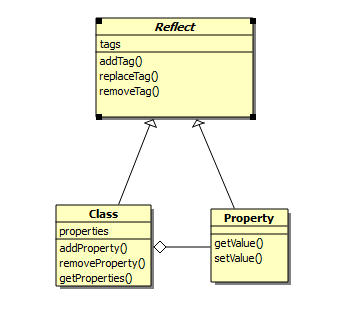
\includegraphics{imagens/reflectDiagram.png}
\caption{Diagrama simplificado das classes de reflex�o}
\label{fig:reflectDiagram}
\end{figure}

Com o uso desta t�cnica conseguimos contornar os dois limitadores impostos pela linguagem C++ para conhecimento e acesso a estrutura de objetos em tempo de execu��o, por�m, ainda temos um problema relacionado com a inser��o do m�todo que retorna o objeto de reflex�o. Ao impormos ao desenvolvedor a necessidade de criar tal m�todo, a biblioteca deixa de ser transparente, pois estamos impondo a implementa��o de uma interface nas classes a serem mapeadas. Para contornar este problema � proposto a cria��o de uma camada de abstra��o atrav�s do uso de macros de registro, simulando o recurso de \textbf{anota��es} existentes na linguagem JAVA. Estas macros em tempo de pr�-processamento do c�digo ser�o expandidas, construindo o m�todo de retorno do objeto de reflex�o. Desta maneira a cria��o do m�todo ser� feita de forma transparente para o desenvolvedor.

No trecho de c�digo \ref{lst:annotationsExample} temos um esbo�o da utiliza��o deste mecanismo. Nas linhas 7 e 13 temos as macros \textbf{ORM4QT{\textunderscore}BEGIN} e \textbf{ORM4QT{\textunderscore}END}, que delimitam o in�cio e final da �rea de especifica��o de mapeamento. A primeira macro ser� expandida gerando a declara��o do m�todo de retorno do objeto de reflex�o e a segunda expandir� o encerramento do m�todo. Todas as macros compreendidas entre elas ir�o expandir o corpo do m�todo. As outras duas macros utilizadas s�o a \textbf{CLASS} que recebe como par�metros uma lista vari�vel de tags, e a macro \textbf{PROPERTY} que recebe o atributo a ser mapeado, seguido de uma s�rie de tags. Estas macros servem para registrar metadados sobre classes e atributos respectivamente.

\begin{algorithm}
\caption{Esbo�o da utiliza��o de macros para registro de metainforma��o}
\label{lst:annotationsExample}
\lstinputlisting[]{codigos/annotationsExample.cpp}
\end{algorithm}

Com este mecanismo definido, as responsabilidades da camada Objeto j� podem ser implementadas. Nas pr�ximas se��es ser�o detalhados os mecanismos a serem utilizados para implementa��o da camada de Armazenamento.

\section{Camada de Armazenamento}
\label{sec:storageLayer}

O objetivo principal de uma biblioteca ORM � abstrair do desenvolvedor a cria��o dos comandos SQL para executar as tarefas de persist�ncia, bem como a comunica��o com o banco de dados. A camada de armazenamento alcan�a este cen�rio a partir da utiliza��o de duas classes. A primeira � a \textbf{\textit{"Repository"}}, que disponibiliza em sua interface m�todos para salvar, atualizar, deletar e carregar registros de objetos no banco de dados. Esta classe oferece a possibilidade do uso de transa��es para garantir que um grupo de opera��es seja executado de forma at�mica. Ela tamb�m tem a responsabilidade de gerenciar a comunica��o com o banco de dados, o que � feito atrav�s da utiliza��o da API disponibilizada pelo m�dulo QtSQL oferecido pelo framework Qt.

A segunda classe � a \textbf{\textit{"SQLProvider"}} que define uma interface para gera��o de comandos em linguagem SQL para a execu��o das tarefas de persist�ncia de objetos. Ela utiliza os objetos de reflex�o disponibilizados pela camada Objeto para construir senten�as de acordo com a inst�ncia de objeto a ser persistida. Esta interface deve ser implementada para cada tipo de SGBD que se deseja utilizar, desta forma a adi��o de suporte da biblioteca para diversos SGBDs se torna uma tarefa mais simples. A classe \textit{"Repository"} utiliza uma implementa��o desta interface para gerar os comandos necess�rios para execu��o de suas tarefas. 

\begin{figure}[!htb]
\centering
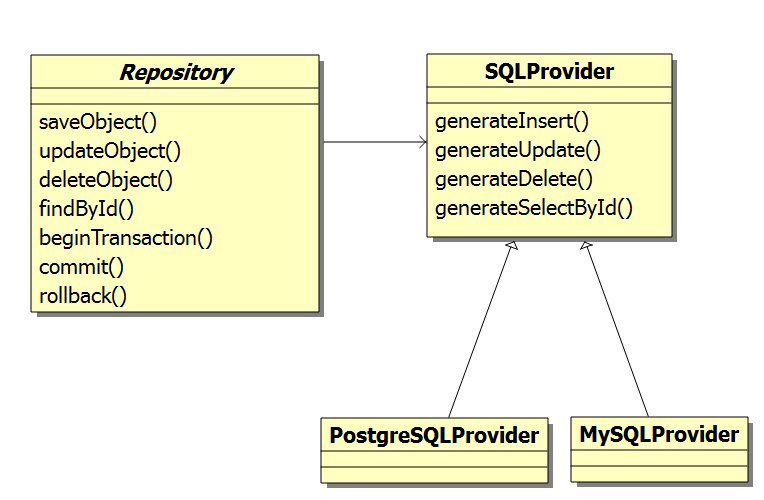
\includegraphics[scale=0.7]{imagens/storageDiagram.png}
\caption{Diagrama de classes simplificado da camada de armazenamento}
\label{fig:storageDiagram}
\end{figure}

Na figura \ref{fig:storageDiagram} temos um esbo�o do diagrama de classes da camada de Armazenamento, onde temos a representa��o de duas poss�veis implementa��es da interface \textit{"SQLProvider"}, uma que daria suporte ao SGBD PostgreSQL e outra ao MySQL. A camada de Armazenamento � menos complexa pelo fato de utilizar a pr�pria camada Objeto e o m�dulo QtSql para facilitar sua implementa��o, por�m ela tamb�m � respons�vel por tratar os erros que podem ocorrer durante a comunica��o com o banco de dados ou execu��o de comandos SQL. Ela deve retornar mensagens bem formatadas descrevendo os erros e oferecer mecanismos para gera��o de logs. 

Com a defini��o desta camada terminamos a especifica��o da biblioteca. A seguir ser� apresentado o cronograma da etapa de desenvolvimento.

\section{Cronograma}
\label{sec:cronograma}

%-------------------------------------------------------------
 %\chapter{Quinto Cap�tulo}
 %\label{cap_quinto}
 %Ap�s a implementa��o da biblioteca ORM4Qt foi necess�rio definir um modelo de testes que pudesse ser aplicado a ela em conjunto com outras bibliotecas j� existentes. O objetivo deste modelo � o de avaliar o n�vel de usabilidade da biblioteca sob o ponto de vista do desenvolvedor, isto �, avaliar a facilidade de uso da biblioteca no ambiente de desenvolvimento utilizado pelo programador.

O modelo de testes escolhido foi o desenvolvimento de uma aplica��o simples chamada ``Minhas Apostilas'', que consiste de um programa que permite o armazenamento de arquivos no formato PDF em uma base de dados. Al�m do arquivo, o aplicativo armazena um pequeno grupo de informa��es referentes a ele, como nome, descri��o e data de altera��o.

Com o intuito de testar a integra��o das bibliotecas utilizadas com o ambiente de desenvolvimento baseado no \textit{framework} Qt com a linguagem C++, o aplicativo utiliza alguns recursos adicionais do Qt para a constru��o de interfaces gr�ficas (m�dulos QtGui e QtWidgets) e para realiza��o de tarefas de forma ass�ncrona (m�dulo QtConcurrent). Al�m disso, o aplicativo foi desenvolvido de forma totalmente port�vel, sendo testado nos sistemas operacionais Ubuntu 14.04 e Microsoft Windows 8.1, ambos com a arquitetura 64 bits.

Foram escolhidas duas bibliotecas ORM existentes para serem comparadas com a biblioteca desenvolvida, sendo elas, a ODB e a QxOrm. Ambas bibliotecas foram descritas no cap�tulo \ref{cap_quarto}.

Nas pr�ximas se��es s�o detalhados os ambientes de desenvolvimento utilizados para realiza��o dos testes e o aplicativo ``Minhas Apostilas'', onde � ressaltado como cada uma de suas funcionalidades foi implementada para cada biblioteca ORM utilizada.

\section{Ambiente de Testes}
\label{sec:ambienteTestes}

A biblioteca ORM4Qt foi desenvolvida utilizando somente componentes oferecidos pelo \textit{framework} Qt vers�o 5.3 e pela especifica��o C++11, portanto ela est� preparada para ser utilizada em qualquer ambiente de desenvolvimento que ofere�a estes componentes. Por�m, neste trabalho somente foram feitos testes nas plataformas Ubuntu vers�o 14.04 64 bits e Microsoft Windows 8.1 tamb�m 64 bits.

Nas duas pr�ximas se��es s�o citados os programas utilizados para compor o ambiente de desenvolvimento de cada uma destas plataformas.

\subsection{Ambiente de Testes Ubuntu 14.04}
\label{sec:testeUbuntu}

Nesta plataforma foram utilizados os seguintes programas para montagem do ambiente de desenvolvimento:

\begin{description}
\item [Compilador \textbf{g++} vers�o 4.8.2:] Consiste de um compilador compat�vel com a especifica��o C++11. Ele foi instalado a partir dos reposit�rios oficiais do sistema;
\item [Bibliotecas do \textit{framework} Qt vers�o 5.3:] Foram instaladas a partir de um instalador obtido no site oficial do projeto Qt\footnote{http://qt-project.org};
\item [QtCreator vers�o 3.2.2:] Ambiente de desenvolvimento integrado instalado em conjunto com as bibliotecas do \textit{framework} Qt;
\item [Compilador \textbf{odb}:] Programa que comp�e o a biblioteca ODB. Ele foi instalado a partir de um instalador oferecido no site oficial do projeto\footnote{http://www.codesynthesis.com/products/odb/};
\item [Bibliotecas \textbf{libodb}, \textbf{libodb-pgsql} e \textbf{libodb-qt}:] Comp�em a biblioteca ODB e s�o necess�rias para utiliz�-la em conjunto com o \textit{framework} Qt e com o SGBD PostgreSql. Estas bibliotecas foram instaladas a partir da compila��o de seus c�digos fontes que tamb�m s�o disponibilizados no site oficial do projeto;
\item [Biblioteca \textbf{boost}:] Dep�ndencia necess�ria para utiliza��o da biblioteca QxOrm. Foi instalada a partir dos reposit�rios oficiais do sistema;
\item [Biblioteca QxOrm:] Foi acoplada no projeto do programa ``Minhas Apostilas'';
\item [Biblioteca ORM4Qt:] Tamb�m acoplada no projeto do programa ``Minhas Apostilas''.
\end{description}

\subsection{Ambiente de Testes Microsoft Windows 8.1}
\label{sec:testeWindows}

Nesta plataforma foram utilizados os seguintes programas para montagem do ambiente de desenvolvimento:

\begin{enumerate}
\item Microsoft Visual Studio 2013 Express que inclui um compilador compat�vel com os elementos da especifica��o C++11 utilizados pelas bibliotecas;
\item Bibliotecas pr�-compiladas do \textit{framework} Qt vers�o 5.3;
\item Ambiente de desenvolvimento integrado \textbf{QtCreator} vers�o 3.2.2;
\item Compilador \textbf{odb} e bibliotecas \textbf{libodb}, \textbf{libodb-pgsql} e \textbf{libodb-qt};
\item Biblioteca \textbf{boost}, necess�ria para utiliza��o da biblioteca QxOrm;
\item Biblioteca QxOrm;
\item Biblioteca ORM4Qt.
\end{enumerate}

%-------------------------------------------------------------
 %\chapter{Sexto Cap�tulo}
 %\label{cap_sexto}
 %O objetivo principal deste trabalho foi mostrar que, a partir da utiliza��o dos novos recursos, sobretudo os de programa��o funcional, propostos pelas novas especifica��es da linguagem C++, � poss�vel construir uma biblioteca de mapeamento objeto relacional com uma interface de configura��o mais amig�vel para o desenvolvedor. Para provar esta teoria foi desenvolvida a biblioteca ORM4Qt, uma biblioteca ORM voltada para utiliza��o integrada ao \textit{framework} Qt.

A biblioteca desenvolvida mostrou-se com um n�vel de facilidade de uso mais alto, sobretudo na parte de configura��o do mapeamento, quando comparada com duas existentes no mercado, a ODB e a QxOrm. Um dos motivos para isso acontecer consiste no mecanismo de reflex�o desenvolvido especificamente para a biblioteca, que permite a configura��o do mapeamento e inser��o de metadados com uma interface bem parecida com o mecanismo de anota��es presente nas linguagens JAVA e C\#.

Apesar de apresentar uma interface de configura��o mais simples, a biblioteca desenvolvida n�o p�de ser comparada diretamente com outras em quesitos como o suporte a mapeamento de mecanismos mais avan�ados da orienta��o a objetos (como heran�a e polimorfismo, por exemplo). Isso se deve ao fato de o suporte a tais mecanismos n�o ter sido desenvolvido por n�o fazer parte do escopo principal do trabalho. Por�m, em futuras vers�es da biblioteca o suporte a tais mecanismos ser� adicionado, e, ent�o poder�o ser efetuados testes de compara��o.

Tamb�m n�o foi comparado o desempenho das bibliotecas em rela��o ao tempo de resposta e utiliza��o de mem�ria, devido tamb�m ao fato da diferen�a da quantidade de mecanismos implementados entre as bibliotecas existentes e a desenvolvida. Por�m, ao utilizar o aplicativo ``Minhas Apostilas'', que foi desenvolvido para fins de testes entre as tr�s bibliotecas, a diferen�a de tempo de resposta � impercept�vel ao usu�rio.

A biblioteca ORM4Qt apresenta potencial para se tornar uma biblioteca ORM t�o completa quanto as utilizadas para testes de compara��o. Para que isso seja poss�vel � preciso ampliar o mecanismo de reflex�o de forma a detectar a utiliza��o de heran�a nas classes mapeadas e reconstruir toda a camada de armazenamento para suportar opera��es no banco de dados que envolvam mais de uma tabela, a��o necess�ria para suportar o mapeamento de composi��o e associa��o. Estas melhorias podem ser implementadas em trabalhos futuros.

Outra sugest�o de trabalho futuro consiste na utiliza��o do mecanismo de reflex�o criado, para implementa��o de mecanismos de serializa��o de objetos para arquivos XML e JSON.

%-------------------------------------------------------------
%\appendix
%\chapter{Nome do Ap�ndice}
%\label{apendiceA}
%Segue a sequ�ncia de comandos utilizados para cria��o do banco de dados utilizado pelo aplicativo de teste.

\begin{verbatim}
create table t_documento
(
  c_codigo bigserial,
  c_nome varchar(200) not null unique,
  c_descricao varchar(1000) null,
  c_ultimaAlteracao timestamp not null,
  c_arquivo bytea not null,
  c_versao smallint not null,
  constraint t_documento_PK primary key (c_codigo)
);
\end{verbatim}


%-------------------------------------------------------------
% --- -----------------------------------------------------------------
% --- Referencias Bibliograficas. (Obrigatorio)
% --- -----------------------------------------------------------------
\cleardoublepage
\bibliographystyle{apalike} %tipo de bibliografia
\bibliography{referencias} % arquivo fonte com a bibilografia

\end{document} %Fim do documento principal.